% !TEX encoding = UTF-8 Unicode
\documentclass[a4j,11pt,report]{jsbook}
\usepackage[dvipdfmx]{graphicx}
\usepackage{tabularx}
\usepackage{fancybox}
\usepackage{ascmac}
\usepackage{amsmath,amssymb,amsthm}
\usepackage{bm}
\usepackage{bmpsize}
\usepackage{here}
\bibliographystyle{ipsjsort}

\setlength{\topmargin}{-1in}
\addtolength{\topmargin}{5mm}
\setlength{\headheight}{5mm}
\setlength{\headsep}{0mm}
\setlength{\textheight}{\paperheight}
\addtolength{\textheight}{-25mm}
\setlength{\footskip}{5mm}

\newcommand{\frontpage}[3]{%
\title{卒業論文\\ \vspace{3em}\\{\huge #1}\\ \\#2\vspace{15em}}%
\author{{\huge 成蹊大学理工学部情報科学科}\\ \\{\huge #3}}%
\date{}
\maketitle
\clearpage
\thispagestyle{empty}

\clearpage
}


\newcommand{\point}[1]{
\begin{itembox}[l]{ポイント}
  #1
\end{itembox}
}

\begin{document}

\frontpage  % 以下の各項目を自分のテーマにあわせて修正する.
{計算問題の特徴分布に基づく類題選出による\leavevmode \\ 自己学習支援}
{Self Learning Support by Automatic Selection of Calculation Exercises based on Feature Distribution of Exercises}
{宮地 雄也}



\chapter*{要旨}
\thispagestyle{empty}

本研究では自然言語処理の技術を人工言語の数式に適応し,分類ができるかどうかを目的とした.またその評価指標として累代選出も行い実際まちがえているのかどうかも検討した.
分散表現で文字の特徴量を抽出したのちその特徴量を用いて数式の分散表現化も行い,式のベクトルを得る.この結果から現在では間違った問題から人をクループ化していたシステムから問題をグループ化してその問題を間違えた人の最適化学習支援を行い,より繊細で効果的な学習が期待できる.
この研究の先には大量の個人情報を扱うアダプティブラーニングにおいて問題から分類できるようになれば,学習データが少なくても十分に効果を発揮することが期待できる.


\tableofcontents
\thispagestyle{empty}
\clearpage
\thispagestyle{plain}
\setcounter{page}{1}

\chapter{序論 \label{ch:introduction}}

\if0
\point{
問題提起を行う.
解く価値があり,簡単には解けず,誰も解いていない問題を扱っていることがわかるようにする.
\begin{itemize}
  \item どういう問題に取り組んだのか?
  \item その問題を解くことがなぜ重要なのか? 社会的意義(有用性)・学術的意義(問題の面白さ)
  \item その問題はどこが難しいのか? なぜこれまで解かれていなかったのか? これまではどうしていたのか?
  \item その問題をどのようなアプローチで解こうとしたのか? なぜそうしたのか?
\end{itemize}
}
\fi

昨今,小・中学生の理系離れが問題視されている.平成30年度全国学力・学習状況調査(全国学力テスト)の結果では平均正答率は小学校では算数Bが51.7\%,中学校数学では47.6\%とどちらも最も低く,ついで国語,理科の順で正答率が低い.
小中どちらとも理系教科の習熟度が低いことを示している.
この要因の一つに,数学は一つの計算方法が様々な分野に横断していくことが一度,苦手を生んでしまったらそこからの分野の理解度が下がり,次の分野での応用がきかないために連鎖的に苦手が蓄積することが原因ではないかと考えた.各単元のちょっとした積み残しが,後々,尾を引いていることが全国学力テストの結果から見て取れる.この状況を打破するには子供一人一人の苦手と向き合い,苦手と感じる前に理解していくしかない.
しかしながら,生徒と向き合うべき教師の労働時間は過酷を極めており,ベネッセ教育総合研究所の調査では小中高の教員の領導時間は増加の一途を辿っていることを明らかにした.
表\ref{tb:teacher_time}は文献\cite{benesse_DateBook}での調査の結果の抜粋である.

\begin{center}
  \begin{table}
    \caption{出勤時刻・退勤時刻・学校にいる時間(平均時間、経年比較(教員年齢別〔公立全体〕))}
    \begin{tabular}{|l|c|r|r|r|r|r|r|} \hline
      & 調査年 & 25歳以上 & 26〜30歳 & 31〜40歳 & 41〜50歳 & 51〜60歳  \\ \hline \hline
      & 2010 & 7:44 & 7:43 & 7:44 & 7:42 & 7:42 \\ \cline{2-7}
      出勤時間 & 2016 & 7:44 & 7:43 & 7:44 & 7:42 & 7:42 \\ \cline{2-7}\hline
      & 2010 & 19:30 & 19:40 & 19:10 & 18:57 & 18:31 \\ \cline{2-7}
      退勤時間 & 2016 & 20:00 & 19:54 & 19:26 & 19:05 & 18:46 \\ \cline{2-7}\hline
      & 2010 & 11時間46分 & 11時間57分 & 11時間26分 & 11時間15分 & 10時間49分  \\ \cline{2-7}
      学校にいる時間  & 2016 & 12時間26分 & 12時間18分 & 11時間46分 & 11時間26分 & 11時間06分 \\ \cline{2-7}\hline
    \end{tabular}
    \label{tb:teacher_time}
  \end{table}
\end{center}

表\ref{tb:teacher_time}によると,教員の労働時間は2010年に比べて2016年の方が各年次とも増加しており,教員のやることが増えている一方で
,主であるはずの教材研究や教務準備に時間が避けていないことを示している.
この状況では先生が生徒一人一人に時間をさき,指導することは難しい現状がつづいている.

この打開策として,IT技術駆使した個人別最適化学習に注目が集まっている,
しかし,教育の情報は,生徒の情報と結びついている個人情報なためオープン化できず,現在でているサービスでは各サービス利用者の利用状況からデータを取得し,その運用に利用しているため一部の王手企業が情報を独占している.
そこで個人の統計データではなく,解く数式の方に着目し,計算式自体の特徴を抽出し,間違えた問題と同様の特徴を持つ問題が復習する類題として最適なのではないかという仮定のもと,本論文では数式の特徴を掴むために自然言語処理の分野で使用される分散表現を適用し,さらに再帰ニューラルネットワークを用いて数式ベクトルを作り出すことを目標とし,そのベクトルを用いて実際に復習問題生成を行った.

\chapter{分散表現\label{ch:Distributed representation}}
自然言語処理ではコンピューターで演算するために各単語を判別するために単語一つ一つをonehotベクトルというものに置き換える.
onehotベクトルとはある語彙数$V$の文章の中の単語$w_{i}$がある時,次元数$V$のベクトルに対し$i$番目の要素のみ1で残りが全て0になっているベクトルのことである(式\ref{onehot}).

\begin{equation}
  \label{onehot}
  \bm{A} = \left(
  \begin{array}{c}
    0 \\
    0 \\
    1 \\
    \vdots \\
    0
  \end{array}
  \right)
  \quad \text{(i = 3 の時)}
\end{equation}


これにより単語一つ一つを別々のベクトルとして区別して表記することができる.
しかしonehotベクトルには問題点があり,一つ目として,ある単語の語彙数$V$が増加すると比例してonehotベクトルの次元$V$も大きくなり,
処理に時間がかかる点がある.また二つ目としてonehotベクトルでは情報が0か1しかないので疎なベクトルができる.疎なベクトルとは次元数が大きくてもそのベクトルの持つ意味が薄いベクトルをさす,
このような問題を解決しようと考えられたのが分散表現である.

分散表現とは疎なonehotベクトルを密な密な実数値をの集合をベクトルとして扱い,その実数値で単語の意味を表そうとする手法である.
これにより疎なベクトルであった単語のベクトルを密な表現ができ,また,密度が上がることでベクトルの次元数を削減することができる.
以下,3手法はその分散表現を得るにあたって機械学習を応用した推論をベースとして編み出された手法である.

\clearpage
\section{Continuous Bag-of-Words Model\label{sec:CBOW}}
Continuous Bag-of-Words Model(以降,CBOWと略記)は文献\cite{SkipCBOW}で提唱された手法で,
ある単語数$\upsilon$の単語列$w_{0},w_{1},w_{2},\dots,w_{\upsilon-2},w_{\upsilon-1},w_{\upsilon}$がある時,単語$w_{t}$が文脈中で前後$m$単語をコンテキスト$C$とする時の前後$m$単語が共に共起する事前確率が増大するように学習するモデルである(図\ref{fig:CBOWimage}).


図\ref{fig:CBOWformula}より$w_{t}$をターゲットにした時の周辺単語$m$個を対象としたときの事後確率は式\ref{cobw同時確率}のように書くことができる.CBOWモデルでは式\ref{cobw同時確率}の最大化問題と見ることができる.
そこでCBOWの損失関数は,単に式\ref{cobw同時確率}の確率に対数を取りマイナスをつけ,最小化問題として解く.
式\ref{cbow_loss}はコーパス全体に拡張した形を示す.



\begin{equation}[tb]
  \label{cobw同時確率}
  \begin{array}{c}
    P(w_{t}|w_{t-m},...,w_{t+m})
  \end{array}
\end{equation}

\begin{equation}
  \label{cbow_loss}
  \begin{array}{c}
    L = -\frac{1}{T} \sum_{t = 0}^T \log P(w_{t}|w_{t-m},...,w_{t+m})
  \end{array}
\end{equation}

\begin{figure}
  \centering
  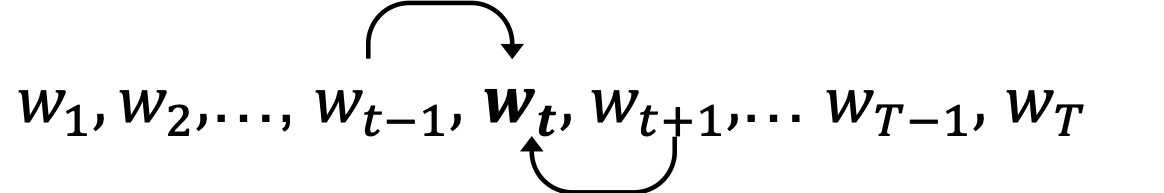
\includegraphics[width = 80mm]{image/cbow_w1w2wt-1wtwt+1.png}
  \caption{単語の列からターゲットとなる単語を推測する($m = 1$)}
  \label{fig:CBOWformula}
\end{figure}

\begin{figure}
  \centering
  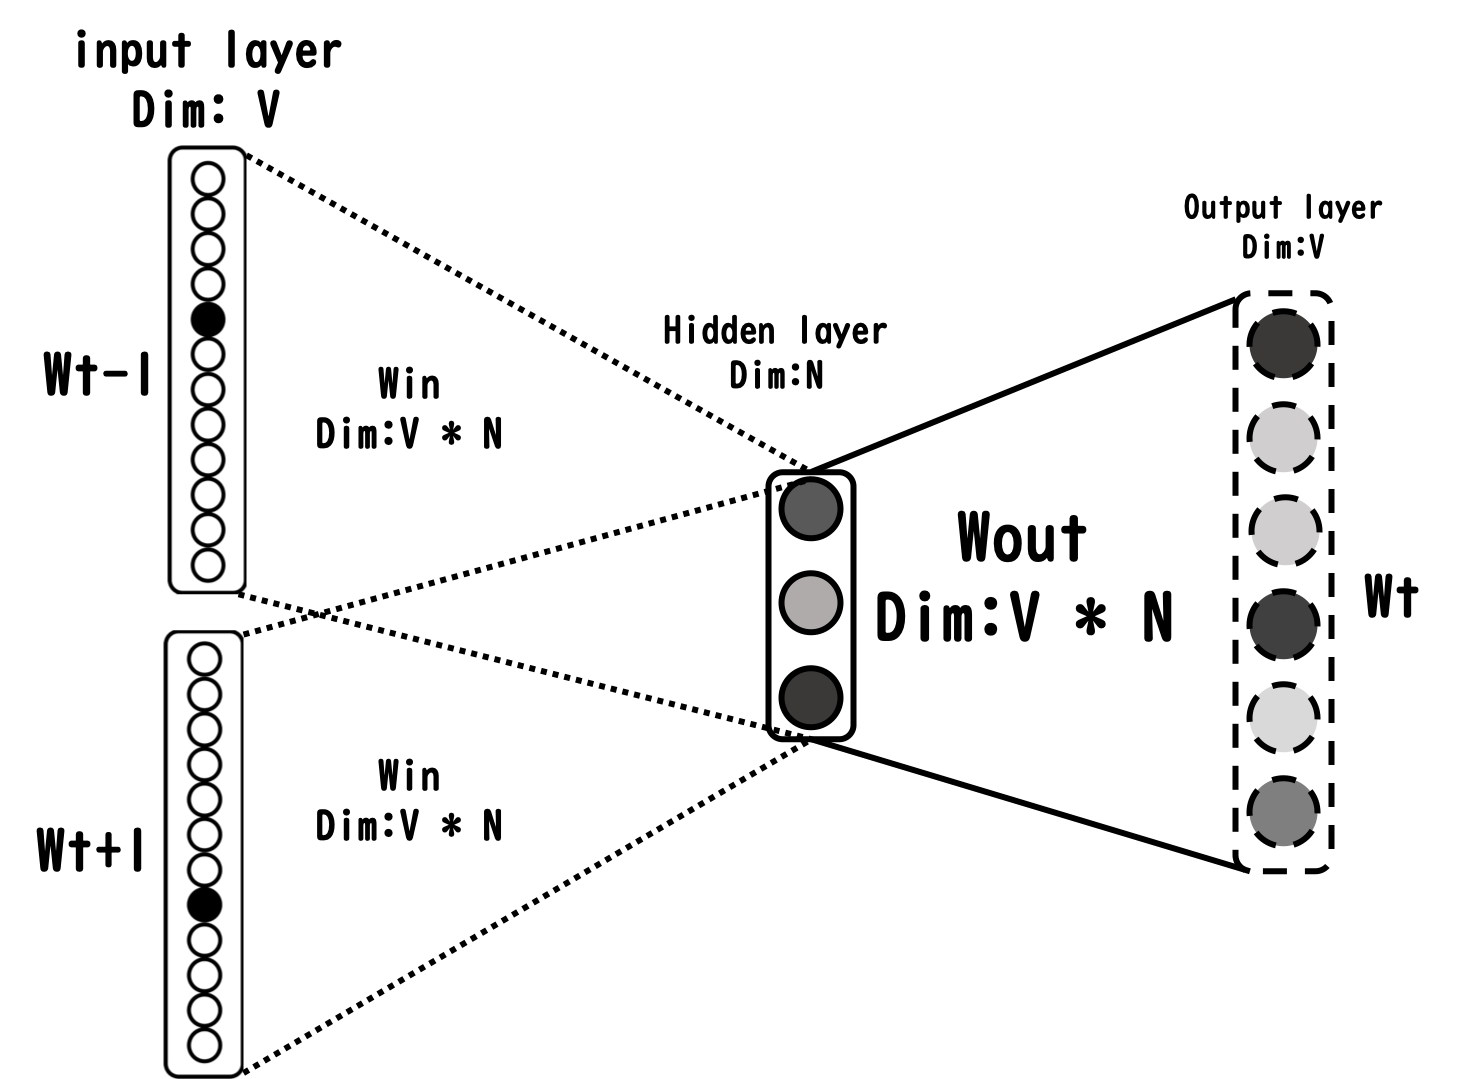
\includegraphics[width = 100mm]{image/CBOW_windowsize_1.png}
  \caption{CBOWのネットワーク構成モデル模式図($ m = 1$) }
  \label{fig:CBOWimage}
\end{figure}


\if0

\begin{figure}
  \centering
  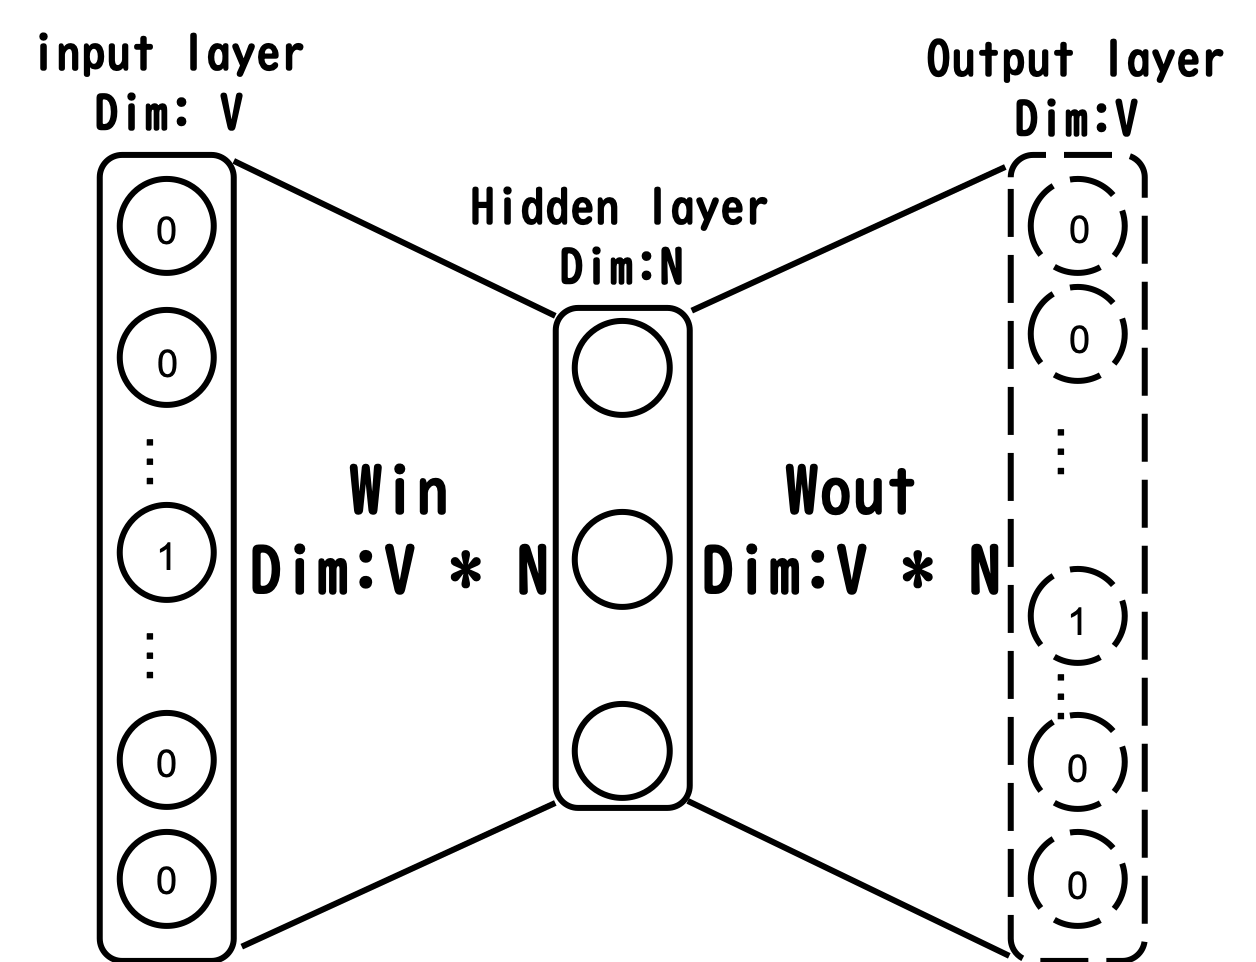
\includegraphics[scale = 0.5]{image/CBOW_image.png}
  \caption{次元圧縮のイメージ図 次元数$v$のベクトルに$V \times N $の埋め込み行列をかけて隠れ層のベクトルの次元を$N$次元に圧縮すことができる}
  \label{fig:CBOWimage}
\end{figure}
\fi

\clearpage

\section{Skip Gram \label{sec:SkipGram}}
Skip Gramは文献\cite{SkipCBOW}で紹介されている章\ref{sec:CBOW}で述べたCBOWとは別の手法である.
CBOWとは逆に中心の単語$w_{t}$から$m$個の周辺単語を推測するモデルである.
ネットワーク構成は図\ref{fig:SkipGramimage}のようになる.

\begin{figure}
  \centering
  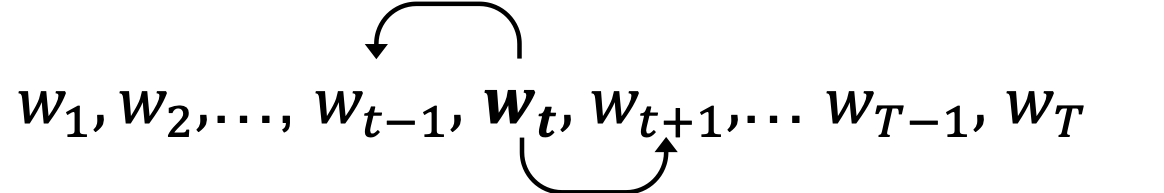
\includegraphics[width = 80mm]{image/skipgram_w1w2wt-1wtwt+1.png}
  \caption{単語の列からターゲットとなる単語を推測する($m = 1$)}
  \label{fig:Skipformula}
\end{figure}


\begin{figure}
  \centering
  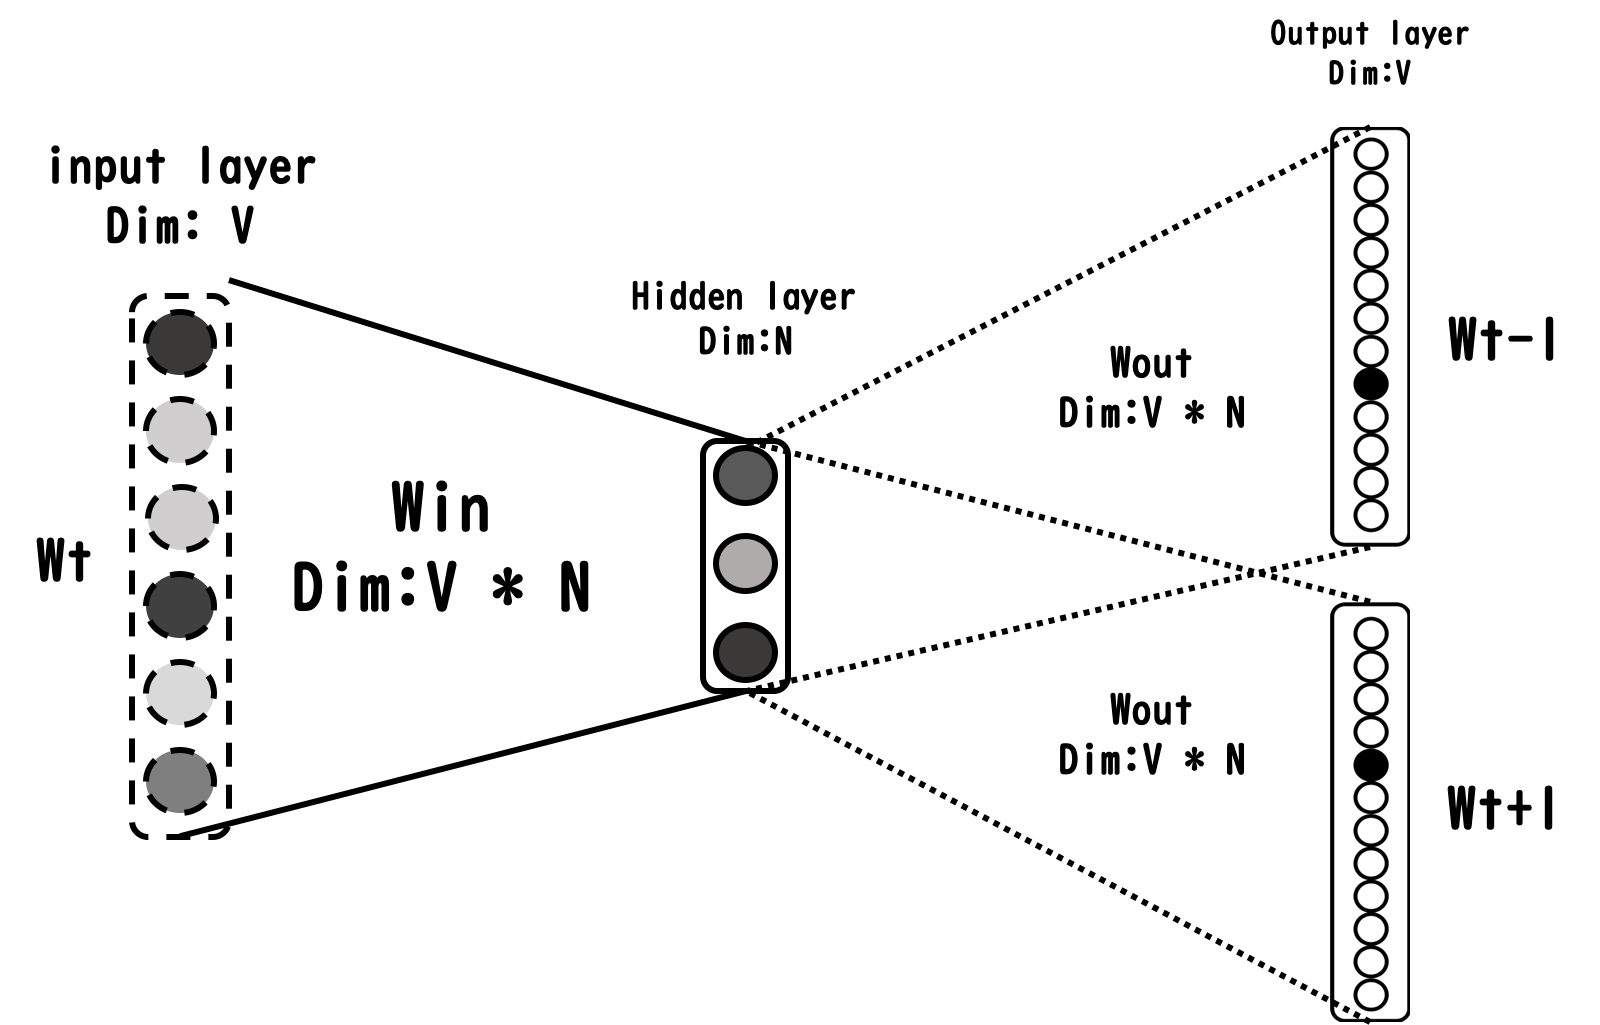
\includegraphics[width = 100mm]{image/SkipGram_windowsize_1.png}
  \caption{SkipGramのネットワーク構成モデル模式図($ m = 1$) }
  \label{fig:SkipGramimage}
\end{figure}



ある単語$w_{t}$が入力層に入力され,周辺単語の$w_{t-m},...,w_{t+m}$を推測する時,その全てが同時に起こる確率は式\ref{skip_probality}となる.

\begin{equation}
  \label{skip_probality}
  \begin{array}{c}
    P(w_{t-m},...,w_{t+m}|w_{t})
  \end{array}
\end{equation}

ここでSkipGramモデルは$w_{t-m},...,w_{t+m}$のそれぞれのあいだに関係性がないと仮定し,交差エントロピーを用いて損失関数(式\ref{skip_lossfunc})を定義する.

\begin{equation}
  \label{skip_lossfunc}
  \begin{split}
    \log P(w_{t-m},...,w_{t+m}|w_{t} ) &= -\log \prod_{k = 0}^m P(w_{t-k}|w_{t})   \\
    &= - \sum_{k = 0}^m \log P(w_{t-k} | w_{t})
  \end{split}
\end{equation}

そして式\ref{skip_lossfunc}をコンテキスト$C$をコーパス全体に拡張すると式\ref{skip_loss}となり,この式を学習によって最小化していく.

\begin{equation}
  \label{skip_loss}
  \begin{split}
    \sum_{C} \log P(w_{t-m},...,w_{t+m}|w_{t} ) &= \sum_{C} -\log \prod_{k = 0}^m P(w_{t-k}|w_{t})   \\
    &= - \sum_{C} \sum_{k = 0}^m \log P(w_{t-k} | w_{t})
  \end{split}
\end{equation}


\chapter{LSTM(Long short-term memory)\label{ch:LSTM}}
順伝播ニューラルネットワークでは前の情報はつかわないため文章や音声など,一つ前の情報に影響を受けるデータに対しては有用ではない.
そこで,ある時刻$t$の出力の際,過去の情報も扱う再帰ニューラルネットワーク(以降 RNN と省略)というものが発案された.
これは時刻$t$の入力を$x_{t}$とする時,各ネットワークは過去の情報を記憶しているようにみなすことができる.
しかしながら通常のRNNの場合,時間が経つほどに前の情報は薄れていく勾配消失が起こることがあった.
これを解決しようとしたのが記憶情報ごとにメモリーの役割を果たすネットワークを分けたLong short-term memory(以降,LSTMと省略)というモデルである.
LSTMでは前の時刻$t-1$の$C_{t-1}$,$h_{t-1}$,$x_{t}$が入力ベクトルとして受け取る.
$C_{t-1}$はLSTMで導入された時刻0からt-1までの情報を記録しているベクトル,$h_{t-1}$は一時刻前の出力ベクトル,$x_{t}$は時刻$t$の入力ベクトルである.
それぞれのセルを計算するために4つのゲートを導入する.それぞれのゲートは入力セルの情報をどれくらい加味するかを重み付けするゲートである.
様々なバージョンがある中でもっとも基本的なネットワーク構成を模式図を図\ref{fig:LSTM_Simple}に示す.以下各ゲートに対して説明する.


\begin{figure}
  \centering
  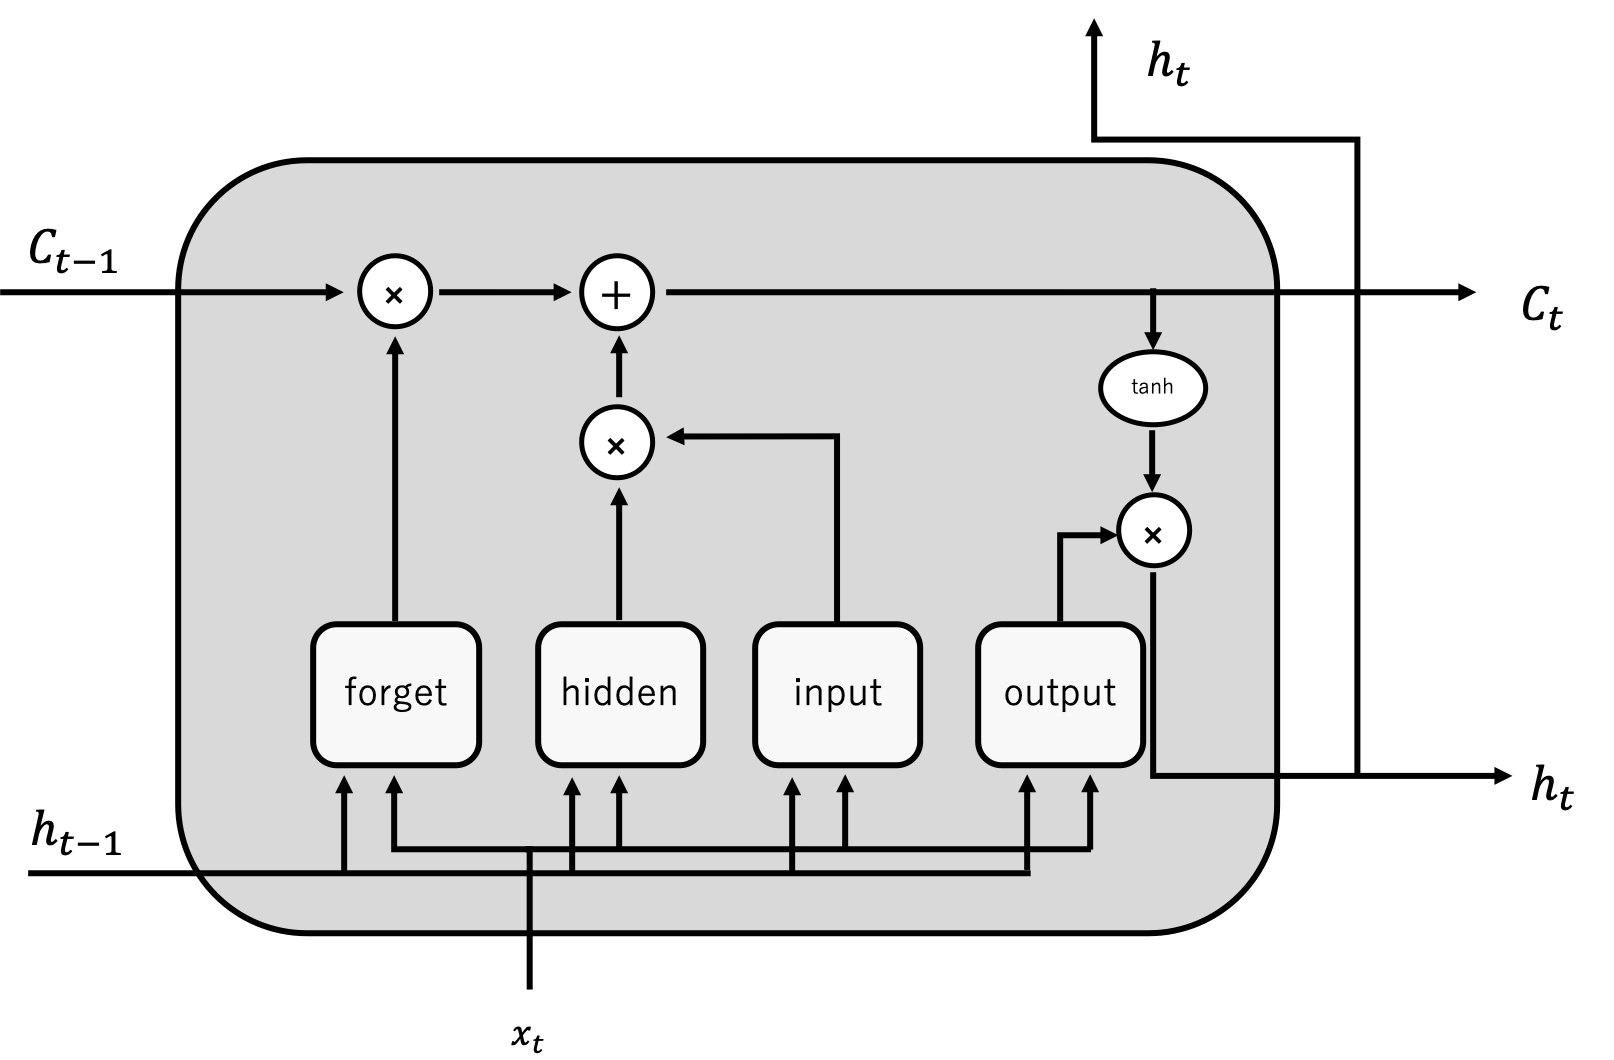
\includegraphics[width = 100mm]{image/lstm_simple_image.png}
  \caption{LSTMのネットワーク構成モデル模式図:図中のforget,hidden,input outputはそれぞれゲートが扱う情報を示している }
  \label{fig:LSTM_Simple}
\end{figure}

\section{forgetゲート\label{sec:forget}}
forgetゲートは過去の情報が詰まっている$C$セルをどの程度次の今の時刻に使うかを決める重みである.
その重みは入力と一時刻前の隠れ層の出力が使われており,その式を\ref{eq:forget}に示す

\begin{equation}
  \label{eq:forget}
  \begin{split}
    f = sigmoid(x_{t}W_{x}^{(f)} + h_{t-1}W_{h}^{(f)} + b^{(f)}
  \end{split}
\end{equation}
これにより時刻$t$の$C_{t}$は式\ref{eq:forgetgate}と求められる.

\begin{equation}
  \label{eq:forgetgate}
  \begin{split}
    C_{t} = f \odot C_{t-1}
  \end{split}
\end{equation}


\section{outputゲート\label{sec:output}}
ouputゲートでは次の時刻にどれくらい現在の情報を渡すかを決める重みである.
その重みは入力と一時刻前の隠れ層の出力が使われており,その式を\ref{eq:output}に示す


\begin{equation}
  \label{eq:output}
  \begin{split}
    o = sigmoid(x_{t}W_{x}^{(o)} + h_{t-1}W_{h}^{(o)} + b^{(o)}
  \end{split}
\end{equation}
これにより時刻$t$の$C_{t}$は式\ref{eq:outputgate}と求められる.

\begin{equation}
  \label{eq:outputgate}
  \begin{split}
    C_{t} = o \odot \tanh(C_{t})
  \end{split}
\end{equation}

\section{hiddenゲート\label{sec:hidden}}

hiddenゲートではforgetゲートで差し引かれた記憶セル$C$に新たな情報を加えるゲートである.

その情報は入力と一時刻前の隠れ層の出力を用いて算出する.(式\ref{eq:hidden})


\begin{equation}
  \label{eq:hidden}
  \begin{split}
    \bar{h} = \tanh(x_{t}W_{x}^{(h)} + h_{t-1}W_{h}^{(h)} + b^{(h)}
  \end{split}
\end{equation}

この$\bar{h}$が一時刻前の$C_{t-1}$に加算されることで新たな記憶を追加する.


\section{inputゲート\label{sec:input}}

inputゲートではhiddenゲートで追加しようとした新たな記憶をどのくらい加算するかを決める重みを求めるゲートである.
その重みは入力と一時刻前の隠れ層の出力が使われており,その式を\ref{eq:input}に示す


\begin{equation}
  \label{eq:input}
  \begin{split}
    i = sigmoid(x_{t}W_{x}^{(i)} + h_{t-1}W_{h}^{(i)} + b^{(i)}
  \end{split}
\end{equation}

これにより時刻$t$の$C_{t}$は式\ref{eq:inputgate}と求められる.

\begin{equation}
  \label{eq:inputgate}
  \begin{split}
    C_{t} = sigmoid (C_{t} + i )
  \end{split}
\end{equation}

\section{LSTMのまとめ}
章\ref{eq:forget},章\ref{sec:output},章\ref{sec:input},章\ref{eq:hidden}で紹介したものをまとめると式\ref{eq:all}のようになる.


\begin{equation}
  \label{eq:all}
  \begin{split}
    f &= sigmoid(x_{t}W_{x}^{(f)} + h_{t-1}W_{h}^{(f)} + b^{(f)} \\
    o &= sigmoid(x_{t}W_{x}^{(o)} + h_{t-1}W_{h}^{(o)} + b^{(o)} \\
    \bar{h} &= \tanh(x_{t}W_{x}^{(h)} + h_{t-1}W_{h}^{(h)} + b^{(h)} \\
    i &= sigmoid(x_{t}W_{x}^{(i)} + h_{t-1}W_{h}^{(i)} + b^{(i)}
  \end{split}
\end{equation}

\begin{equation}
  \label{eq:all2}
  \begin{split}
    c_{t} &= f \odot c_{t-1} + g \odot i
  \end{split}
\end{equation}

\begin{equation}
  \label{eq:all3}
  \begin{split}
    h_{t} &= o \odot \tanh(c_{t})
  \end{split}
\end{equation}

LSTMモデルを3時刻分展開したものを図\ref{fig:LSTM_3timeconcat}に示す.

\begin{center}
  \begin{figure}
    \centering
    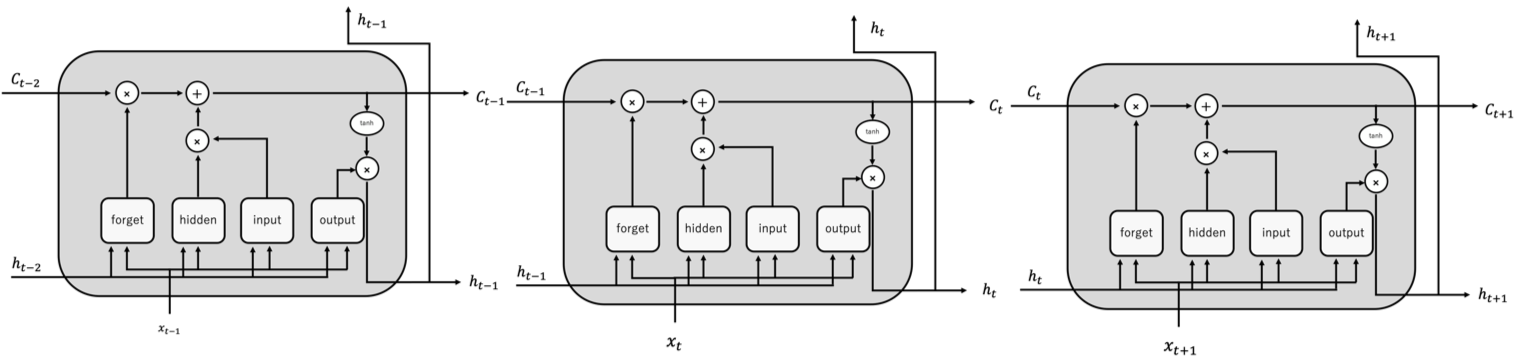
\includegraphics[width=\linewidth]{image/LSTM_concat.png}
    \caption{LSTMの3時刻展開:記憶を守る機構によりより高い濃度で次の時刻に情報を渡すことができる}
    \label{fig:LSTM_3timeconcat}
  \end{figure}
\end{center}






\chapter{系列変換\label{ch:Seq2Seq}}

系列変換とは再帰ニューラルネットワークを用いて時系列データを時系列データに変換することをさす.
モデルの構成図の例を図\ref{fig:seq2seq_3time}にしめす.

\begin{center}
  \begin{figure}[tbh]
    \centering
    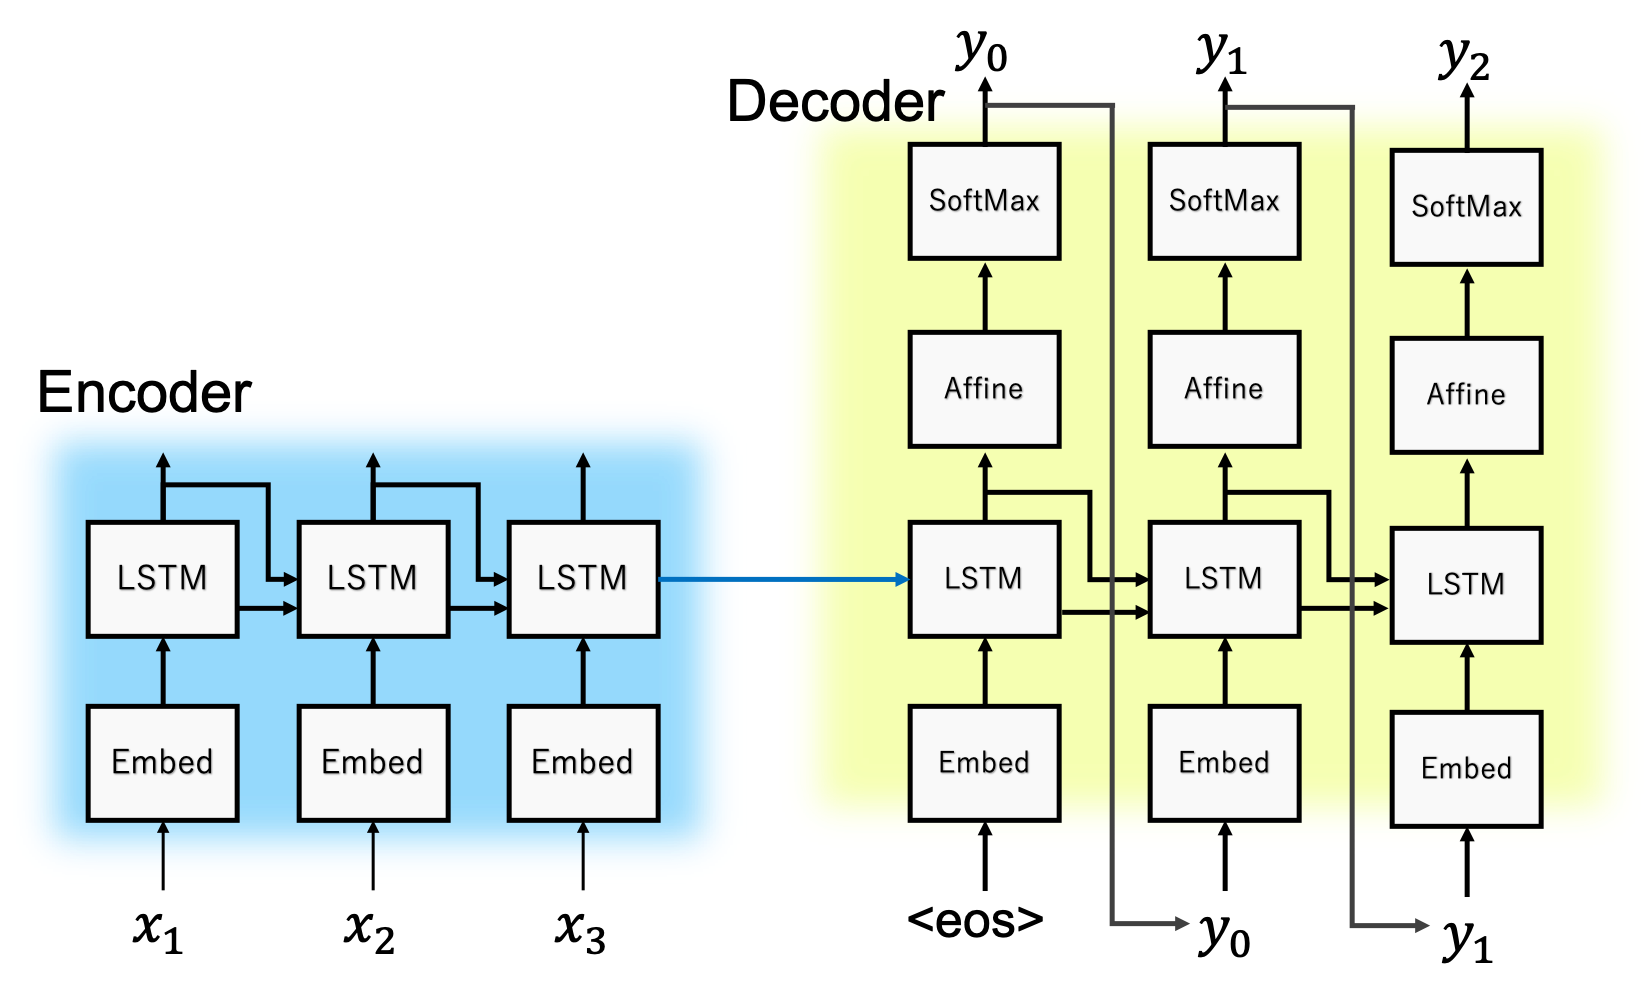
\includegraphics[width=\linewidth]{image/seq2seq_image.png}
    \caption{LSTMを用いた基本的な系列変換モデルの3時刻展開 }
    \label{fig:seq2seq_3time}
  \end{figure}
\end{center}

大きく分けてEncoderとDecoderに分かれる.Encoder側は入力を受け取りEmbedding層で入力系列$x_{i}$を埋め込み行列に変換し,
LSTMに入力として渡す.EncoderではLSTMが時系列データを記憶するメモリーのように振る舞い次の時刻へ情報を渡していく,
時刻$t$の時のLSTMの隠れ層の出力$h_{t}$にはLSTMが渡してきた$1 \sim t$までの情報が溜め込まれており,入力系列を変換するために必要な情報が
エンコードされて任意の固定長ベクトルに溜め込まれる.
この固定長ベクトルDecoder側の最初のLSTMの前の時刻の$h$として入力され,区切れ文字<eos>を入力として受け取り,
エンコーダー側と同じように埋め込み行列に変換しLSTMで再帰的に学習,そしてAffine層で入力ベクトルの大きさと同サイズに圧縮し,
SoftMax層(式\ref{eq:softmax})でベクトルの値を確率に変換する.

\begin{equation}
  \label{eq:softmax}
  \begin{split}
    softmax(x_{i}) = \frac{ e^{x_{i}} }{ \sum e^{x_{i}} }
  \end{split}
\end{equation}

区切れ文字<eos>によって出力された$y_{0}$を次の時刻の入力とし,$2$時刻目として$y_{1}$を出力し再び区切れ文字を出力するまで繰り返す,
この技術を応用して機械翻訳など時系列データの変換に用いる.


\chapter{Attention\label{ch:attention} }
章\ref{ch:Seq2Seq}で導入した系列変換モデルだが,問題点があり,図\ref{fig:seq2seq_3time}で示したように,系列を固定長のベクトルに情報を溜め込むのだが,系列が長くても短くても固定長のベクトルになるため長い系列だと容量不足になる問題があった.
そのことを解決する手法の一つとしてAttentionを導入する.
Encoderの出力は時刻$t$の入力系列をベクトルに変換したものなので時刻$t$の出力がもっとも時刻$t$の状態を反映した物であるという仮定のもと,
AttentionではDecoder側で出力系列を生成するとき,出力と対応するEncoderの出力ベクトルに注意して生成するようにする.
これをAttention(注意機構)という.
章\ref{ch:Seq2Seq}の図\ref{fig:seq2seq_3time}にAttentionを加えたネットワークを図\ref{fig:Attention_3time}に示す.




\begin{center}
  \begin{figure}[h]
    \centering
    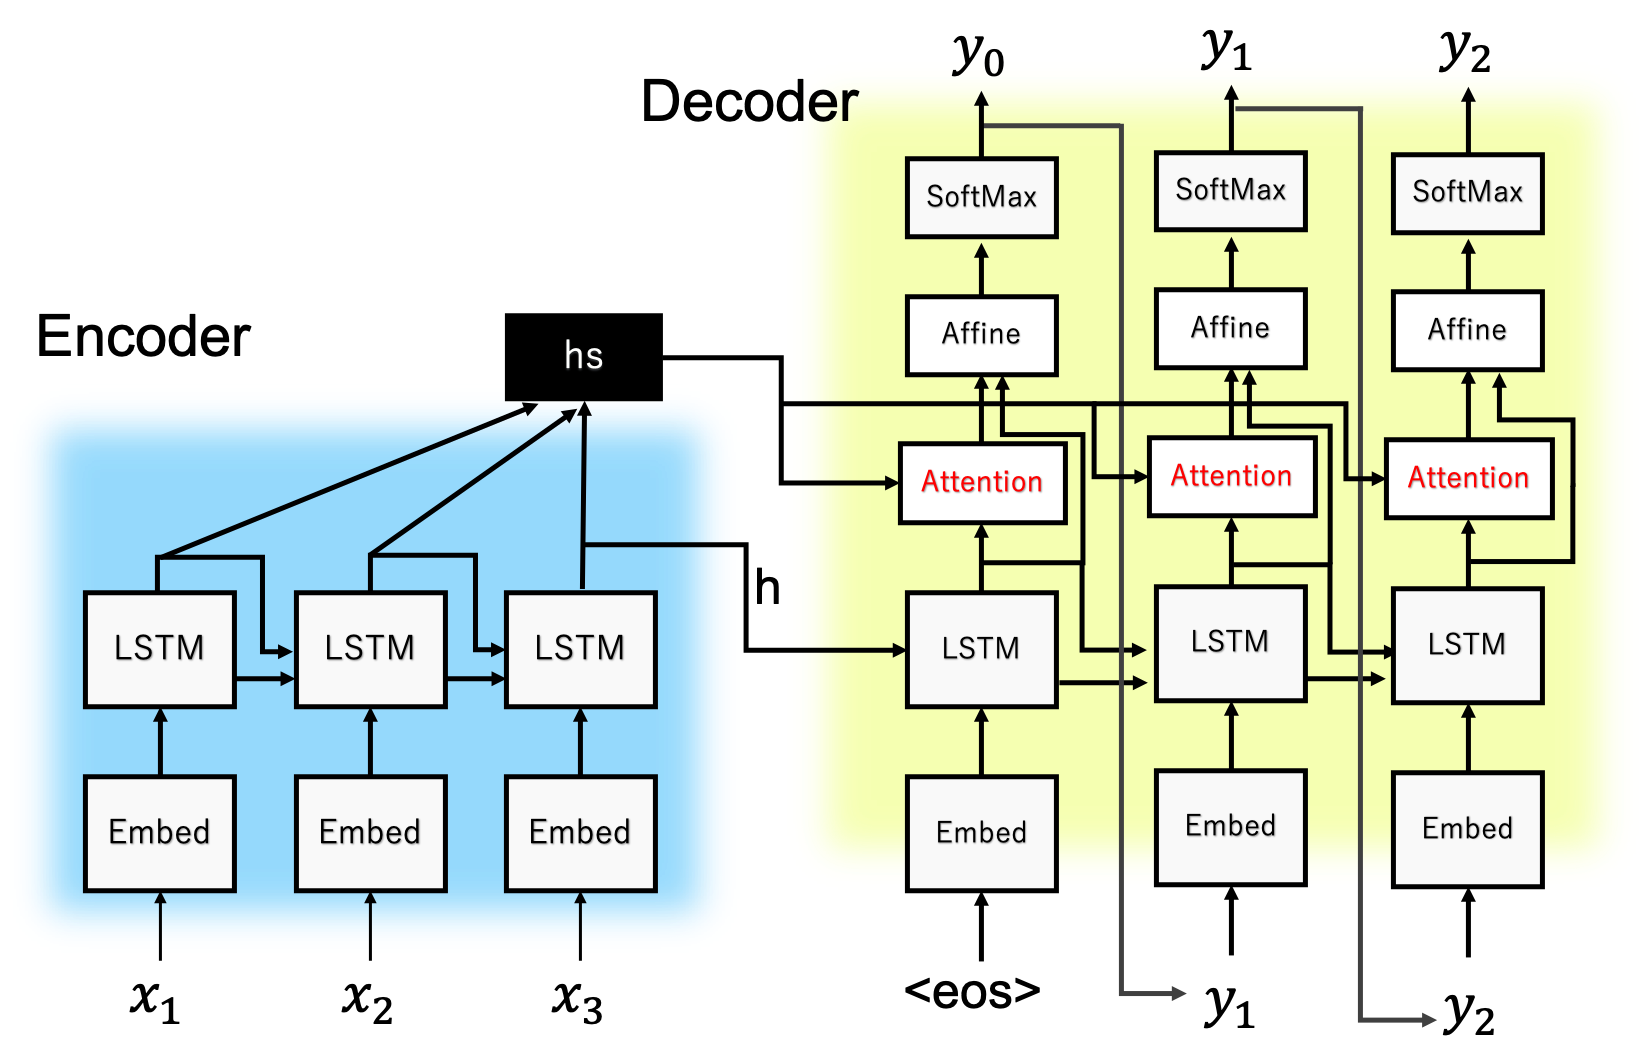
\includegraphics[width=\linewidth]{image/attention_image.png}
    \caption{LSTMを用いた基本的な系列変換モデルの3時刻展開にAttenitonを追加したネットワーク }
    \label{fig:Attention_3time}
  \end{figure}
\end{center}



Encoder側では各時刻の出力を$hs$として溜め込んでいく.
Decoder側ではLSTNを抜けた隠れ層の出力ベクトルを$h^{decoder}$とすると図\ref{fig:Attention_3time}で行うAttentionの計算の概要を
図\ref{fig:Attention_layer}に示す.
Attention Weightはhsと$h^{decoder}$のベクトルの類似度を計算する.その過程を式\ref{eq:AttentionWeight}に示す.

\begin{equation}
  \label{eq:AttentionWeight}
  \begin{split}
    s = hs \odot h^{decoder}  \\
    a = softmax(s)
  \end{split}
\end{equation}

二つのベクトルを内積をとることにより類似度に変換し,その後SoftMax(式\ref{eq:softmax})で変換する.この類似度のベクトルをScoreともいう.

またWeight SumではこのScoreを元にhsのどこに注意を置くのかを算出する.その過程を式\ref{eq:WeightSum}に示す.
よってContextVecterはEncoderの入力系列の重要なところを注視したベクトルが作られ,これをDecoderのLSTMの出力値とconcatし読み込むことでその性能を格段に向上させることに成功している.(文献\cite{attention})


\begin{equation}
  \label{eq:WeightSum}
  \begin{split}
    c = \sum_{i} hs_{i} a_{i}
  \end{split}
\end{equation}

\begin{center}
  \begin{figure}[ht]
    \centering
    \includegraphics[width=0.5\linewidth]{image/attention_layer.png}
    \caption{Attention内部で行う計算  Attention Weightはベクトルの類似度を計算し,Weight Sumは類似度からhsをどれくらい重要視するかを示すContextVecterを算出する}
    \label{fig:Attention_layer}
  \end{figure}
\end{center}


\chapter{Exericises Vecter Representation\label{ch:method}}
\if0
\point{
自分の提案する解決方法を説明する.
\begin{itemize}
  \item 章題は適切なものに変えること.章をわけてもよい.
  \item 必ず具体例を用いること.
  \item 最初に問題を解く上で最も難しい点とそれを解決するアイデアを示す.
  \item 詳細については,全体の流れを示した後,各ステップについて説明する.
  \item 検討時に行った予備評価の結果があれば示す.
\end{itemize}
}
\fi

\section{システム全体の流れ}

数式の特徴を取り出し$S$次元のベクトルに変換し,その分布から類題選出を行うシステムを作成し概要を図\ref{fig:EVS_Simple}に示す,
以下,各システムの箇所ごとに説明する.


\begin{center}
  \begin{figure}
    \centering
    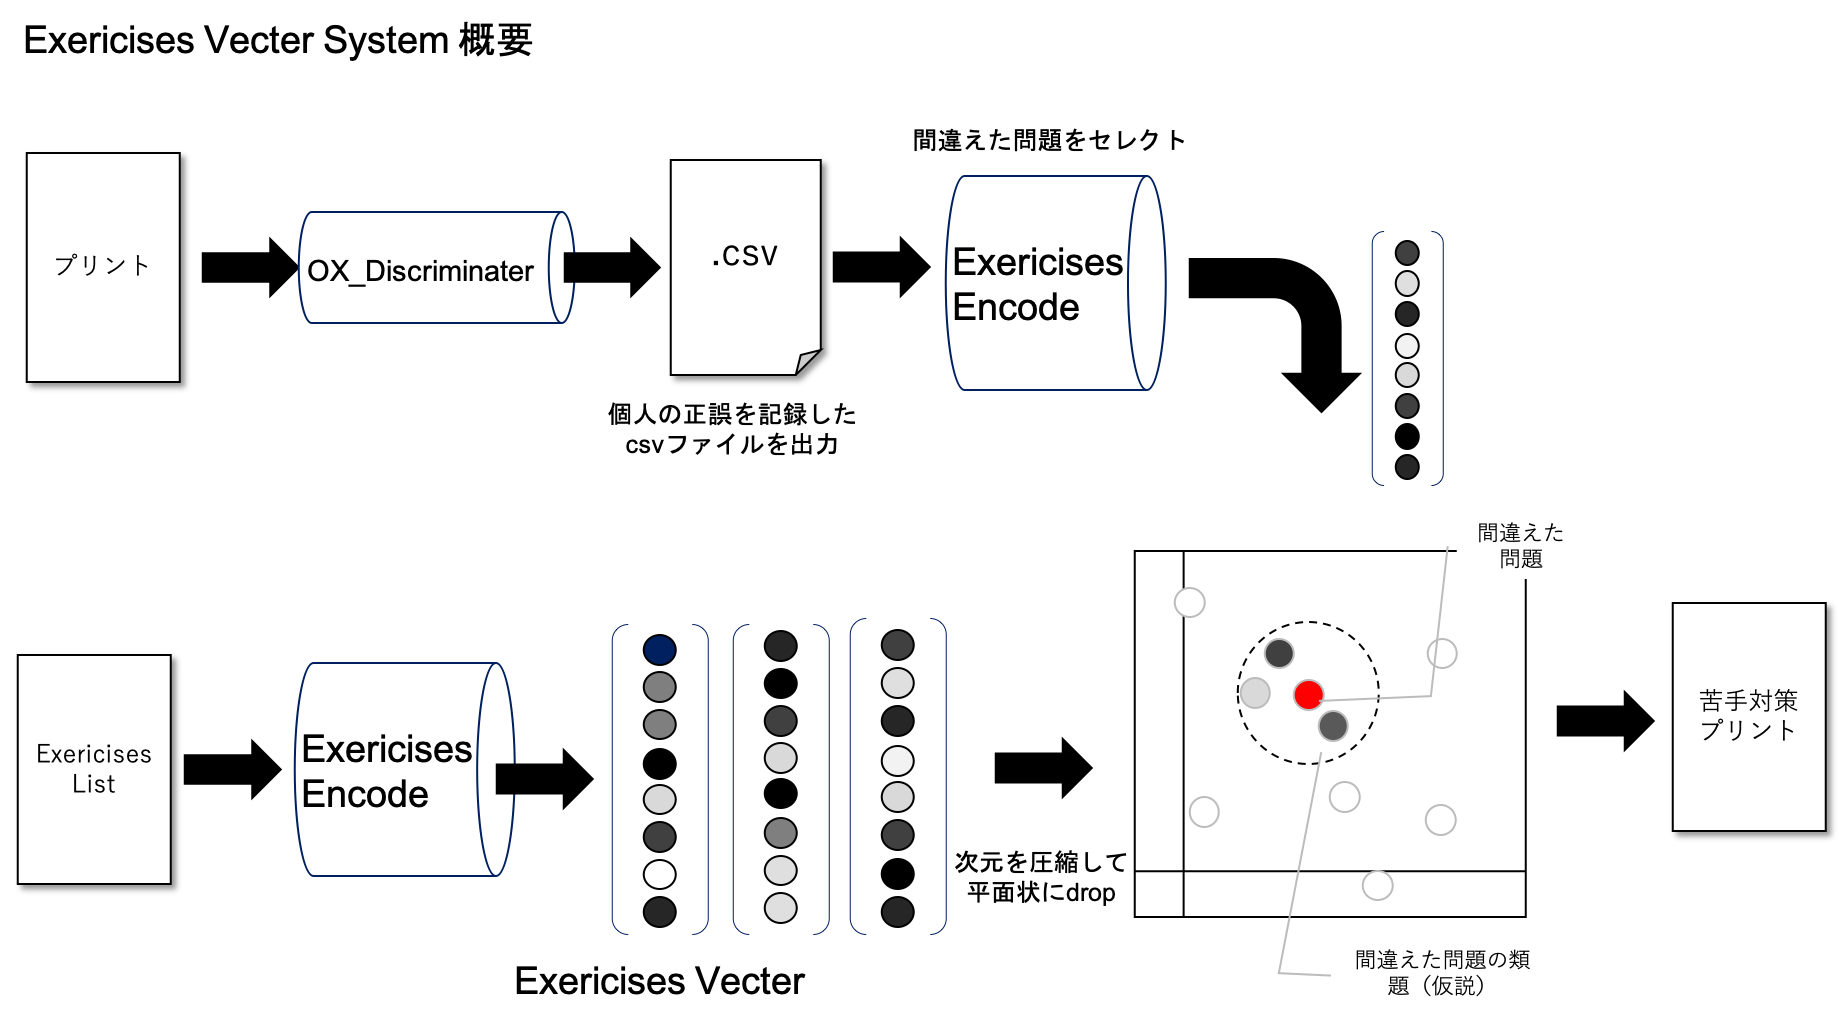
\includegraphics[width=\linewidth]{image/EVS_Simpie.png}
    \caption{LSTMの3時刻展開:記憶を守る機構によりより高い濃度で次の時刻に情報を渡すことができる}
    \label{fig:EVS_Simple}
  \end{figure}
\end{center}

\section{計算式の特徴量抽出}
\subsection{概要}
数式を分布化する際,そのベクトルの中に数式の特徴を入れ込んだベクトルを生成する手法が確立していない.そこで本論文では数式の各文字,記号を単語のようにみなし,onehotベクトルを作成し,それを埋め込み層で特徴を踏まえた低次元ベクトルに変換したのち,系列変換モデルで読み込むことで低次元で数式の特徴を掴んだベクトルを生成できないかと考えた.

この考えを実現するために数式は我々が目にする$2x+3=5$, $\frac{3x-1}{2}+4=\frac{2}{5}$ではなく,テキスト化かつその特徴を強く受けた形に変換する必要がある.
そこで本論文では数式をある一定のルールの中でテキスト化されている{\TeX}形式の数式を用いる.
上記の計算式なら\verb#2x+3=5#,\verb#\frac{3x-1}{2}+4=\frac{2}{5}#とし,このテキストデータを用いて文字単位の埋め込んだベクトルを作成する.

実験を行った手法は以下の2種法で行い,それぞれ分布をpythonを用いて確認した.
\begin{itemize}
  \item CBOW
  \item SkipGram
\end{itemize}

onehotベクトルの置き方は以下の2手法を試し,それぞれPCAとT-SNEで2次元に落としplotし状況を確認する予備実験を行った.
\begin{itemize}
  %  \item $[0,1,2, ... ,9,+,-,=,x ...]$ のように各数字,各記号に割り当てる方法
  \item 出てきた数字,数式の塊をonehotを置く方法($[0,1,2, ... 3.6,0.11,...=.+,-]$)
  \item 3桁までの数字,数式に現れる記号
\end{itemize}


\subsection{文字分布の予備実験結果}
予備実験としてCBOW,SkipGramで文字の特徴が得られているかを確認した.
以下その結果である.

\begin{center}
  \begin{figure}[H]
    \centering
    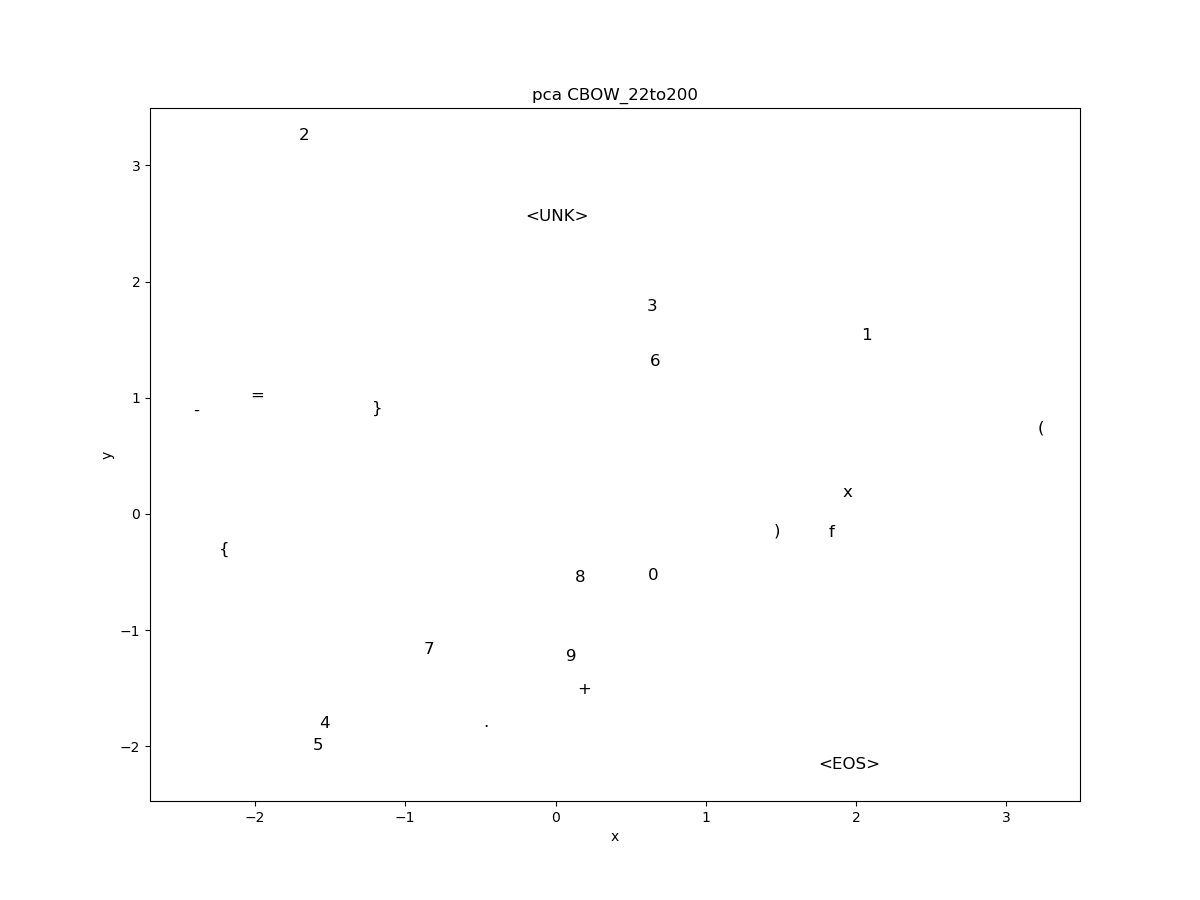
\includegraphics[width=\linewidth]{image/CBOW_pca_out22_200.png}
    \caption{CBOWにて22次元を200次元に分散表現を変換したのちpcaで再構成しグラフ化した結果}
    \label{fig:89x2cbow_pac}
  \end{figure}
\end{center}


\begin{center}
  \begin{figure}[H]
    \centering
    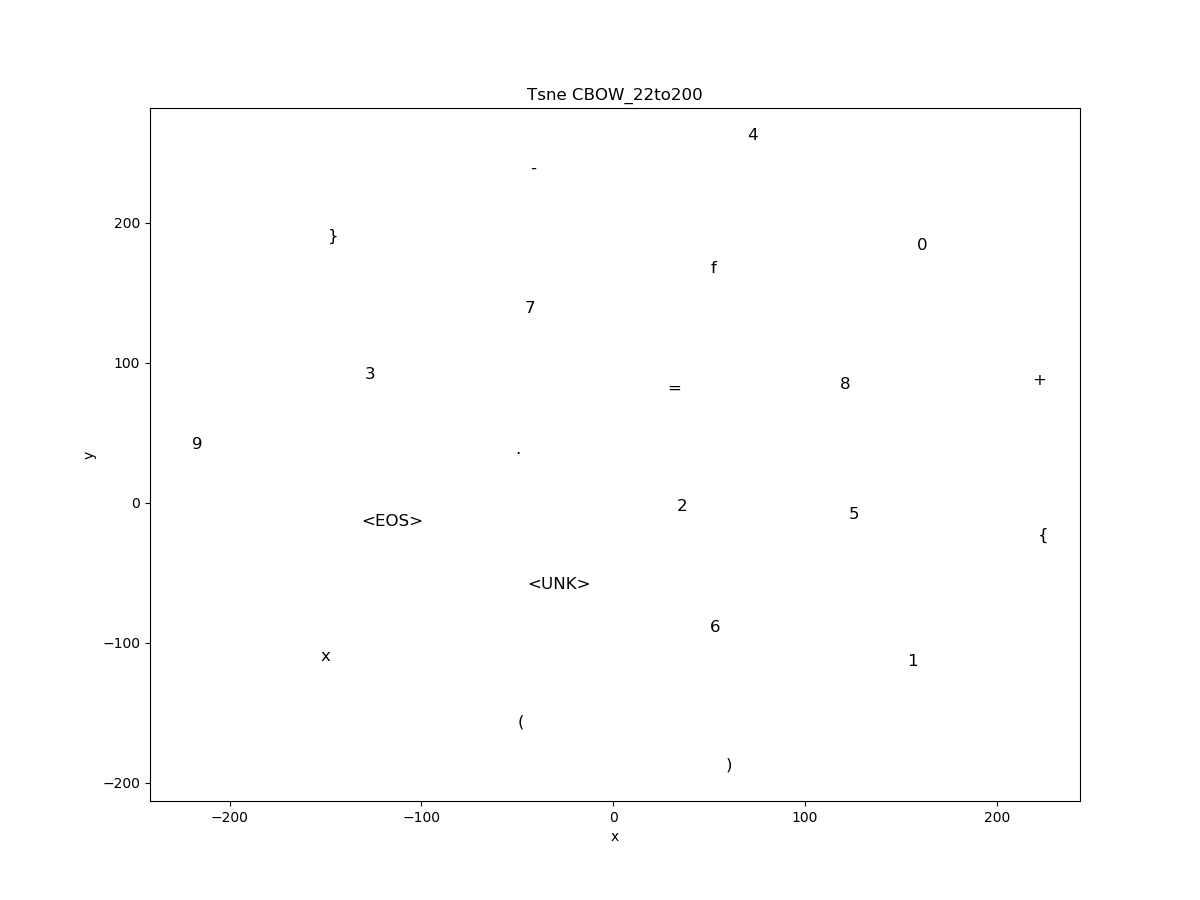
\includegraphics[width=\linewidth]{image/CBOW_tsne_out22_200.png}
    \caption{CBOW 22次元を200次元に分散表現を変換したのちT-SNEで再構成しグラフ化した結果}
    \label{fig:89x2cbow_tsne}
  \end{figure}
\end{center}

図\ref{fig:89x2cbow_pac}や図\ref{fig:89x2cbow_tsne}を見るとそれぞれの文字に関係はないように見える.
しかし,実際にベクトルの類似度のランキングは以下のようになった


\begin{figure}[htpb]
  \centering
  \begin{tabular}{c}
    \begin{minipage}{0.47\hsize}
      \centering
      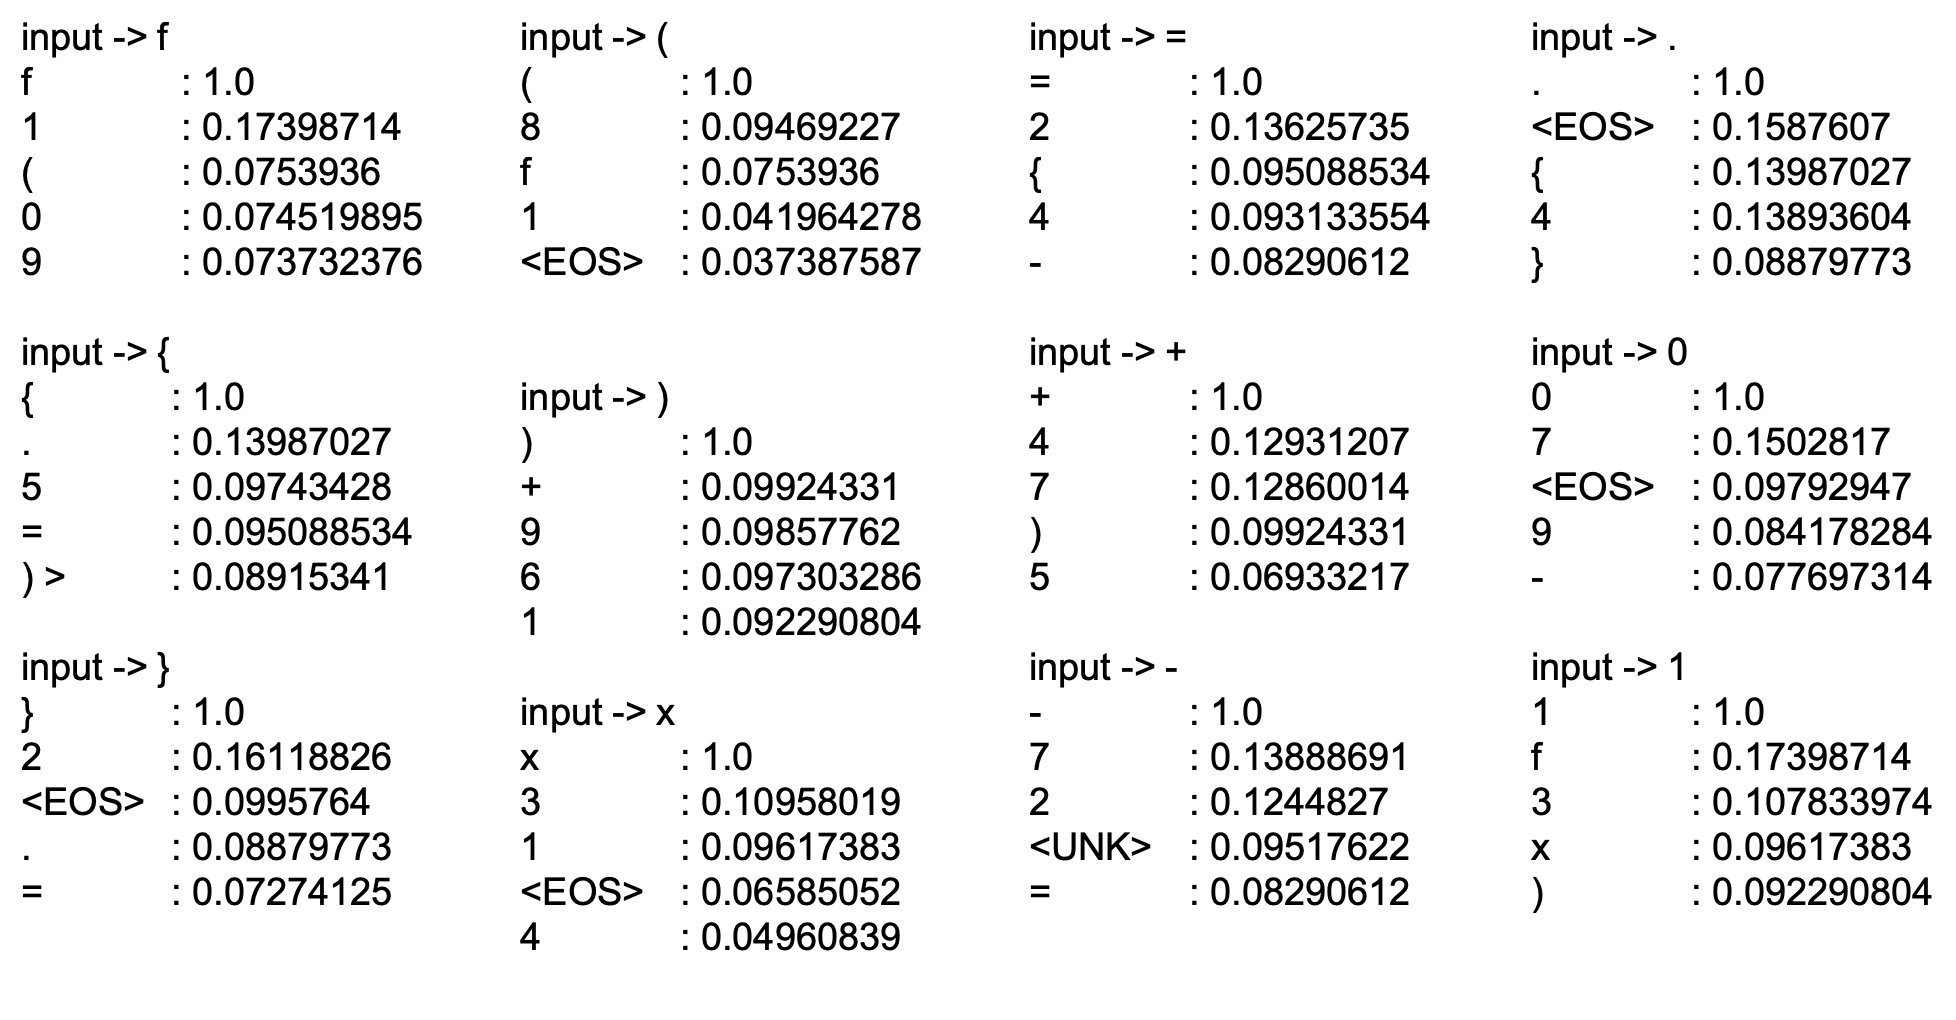
\includegraphics[width=\linewidth]{image/1.png}
    \end{minipage}

    \begin{minipage}{0.06\hsize}
      \hspace{2mm}
    \end{minipage}

    \begin{minipage}{0.47\hsize}
      \centering
      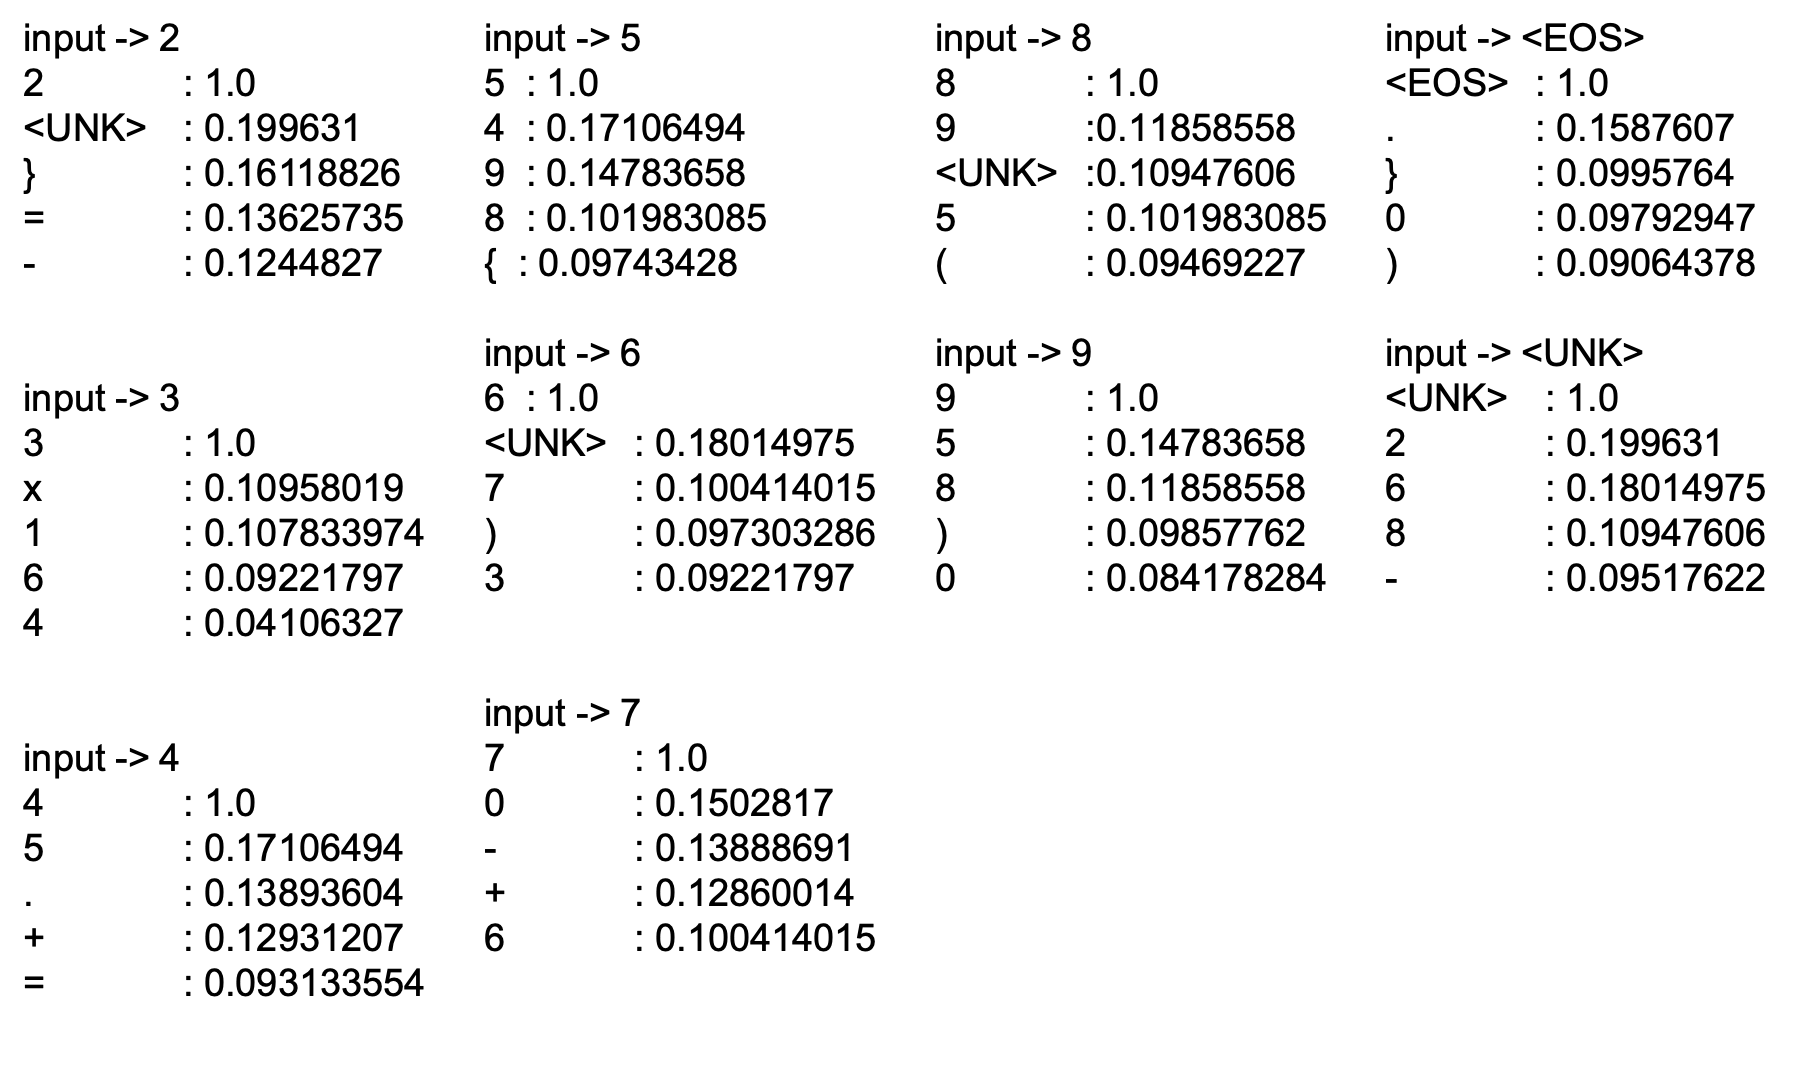
\includegraphics[width=\linewidth]{image/2.png}

    \end{minipage}

  \end{tabular}
  \caption{Seq2Seq}

  \label{fig:textresult}
\end{figure}



\section{系列変換モデルの検討}
本論文の目的としては系列変換の過程で用いれるEncoderからDecoderに渡す最終出力$h$を式ベクトルとしてみなす.
よって$h$の制度を高めていくモデルが必要となる.
実験するモデルは通常のLSTMで行う系列変換,双方向RNNを用いたbi-directionlモデル,通常Decoderが側で利用されるSkipConnectionの三種類をEncoderのモデルとした.
デコーダ側は通常のLSTMで行う系列変換とAttentionを用いたモデルの2種類で確認を行うこととした.
以下モデルを模式図にした.


\begin{figure}[htpb]
  \centering
  \begin{tabular}{c}

    \begin{minipage}{0.47\hsize}
      \centering
      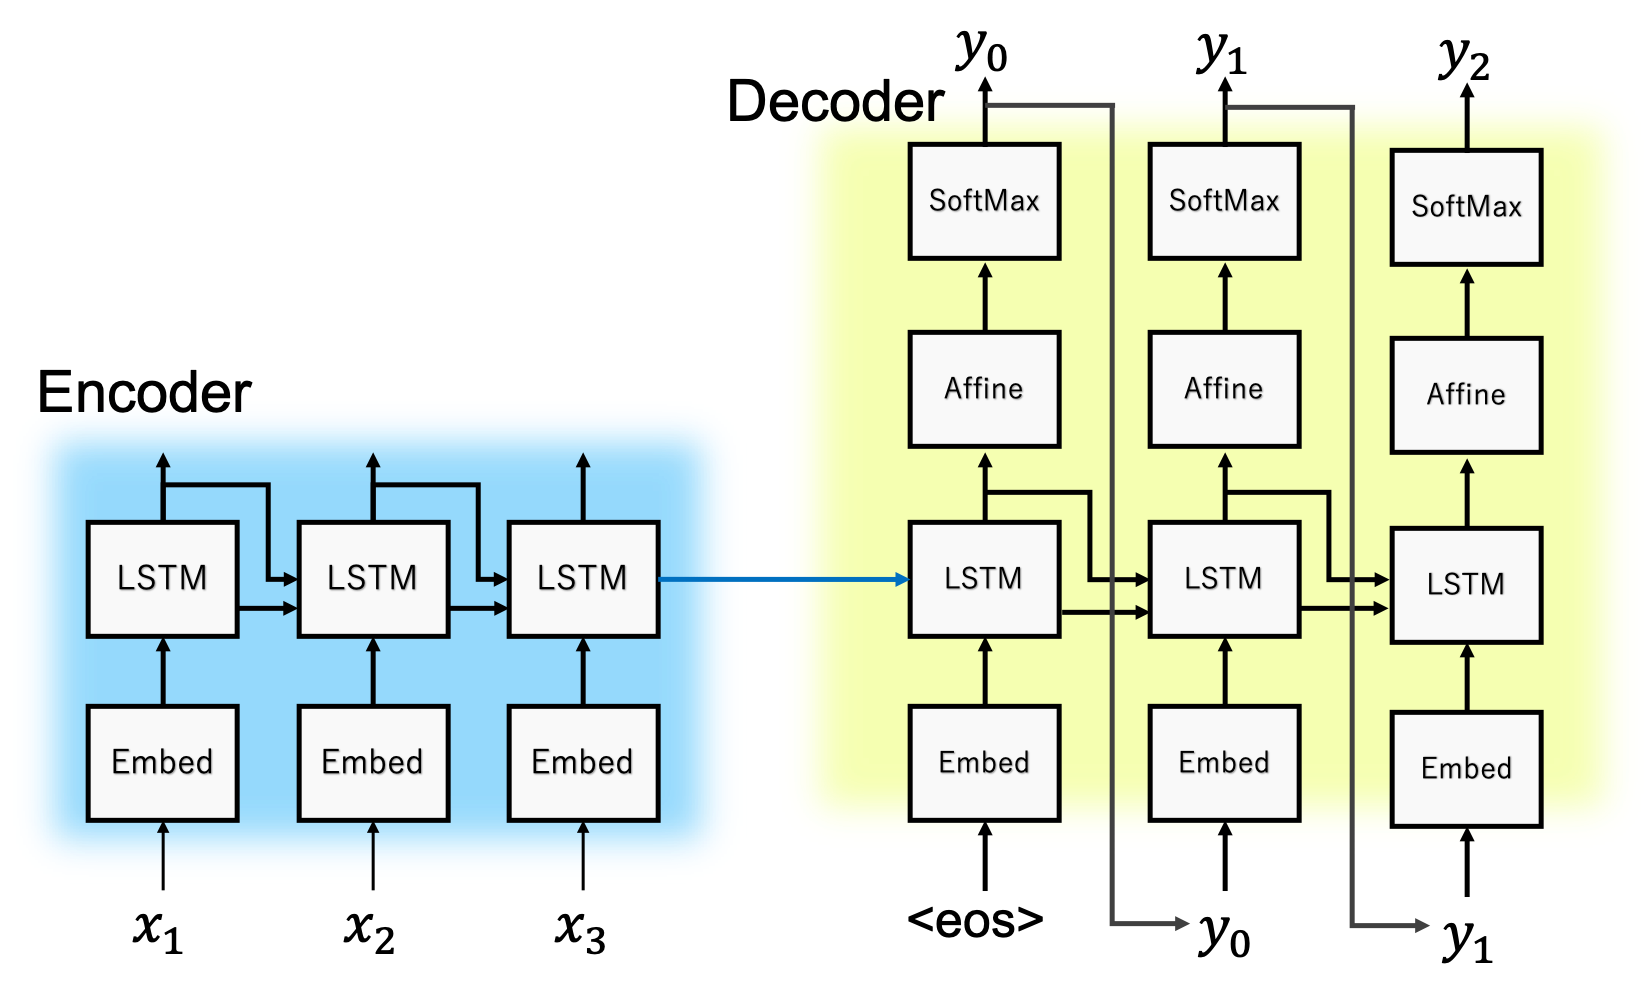
\includegraphics[width=\linewidth]{image/seq2seq_image.png}
      \caption{Seq2Seq}
      \label{fig:seq2seq}
    \end{minipage}

    %--- 中央スペース

    \begin{minipage}{0.06\hsize}
      \hspace{2mm}
    \end{minipage}


    \begin{minipage}{0.47\hsize}
      \centering
      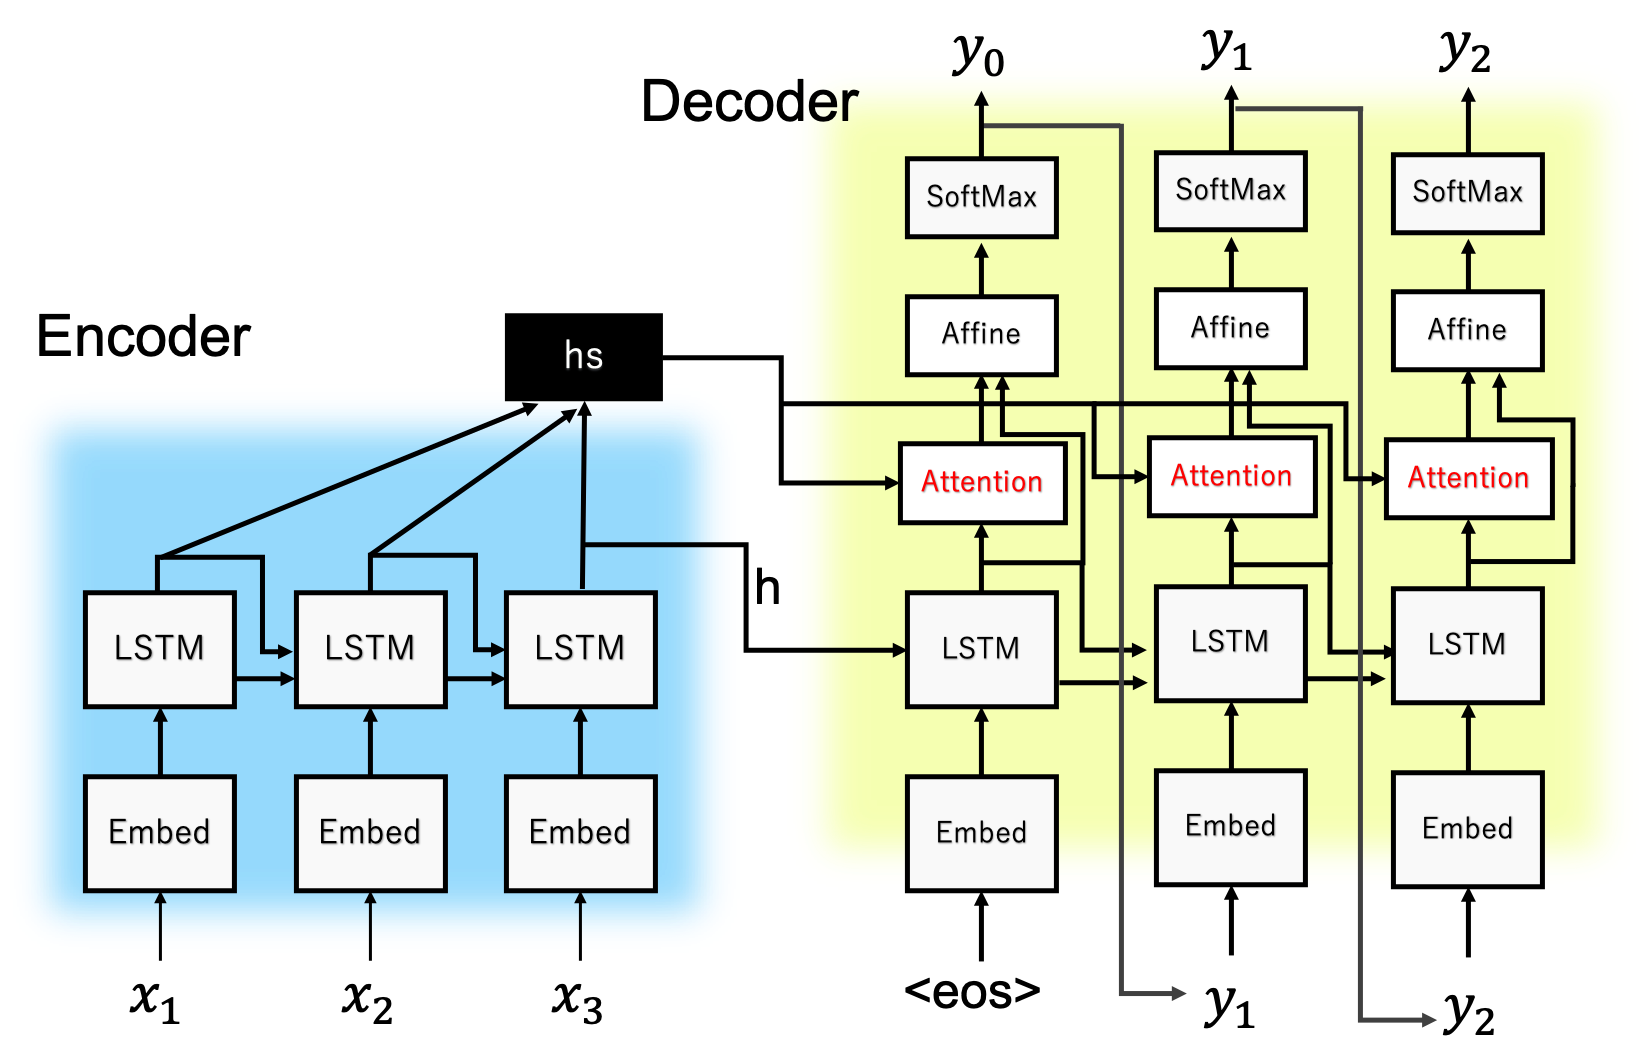
\includegraphics[width=\linewidth]{image/attention_image.png}
      \caption{Attention Seq2Seq}
      \label{fig:Attention Seq2Seq}
    \end{minipage}

  \end{tabular}
\end{figure}


\begin{figure}[htpb]
  \centering
  \begin{tabular}{c}

    \begin{minipage}{0.47\hsize}
      \centering
      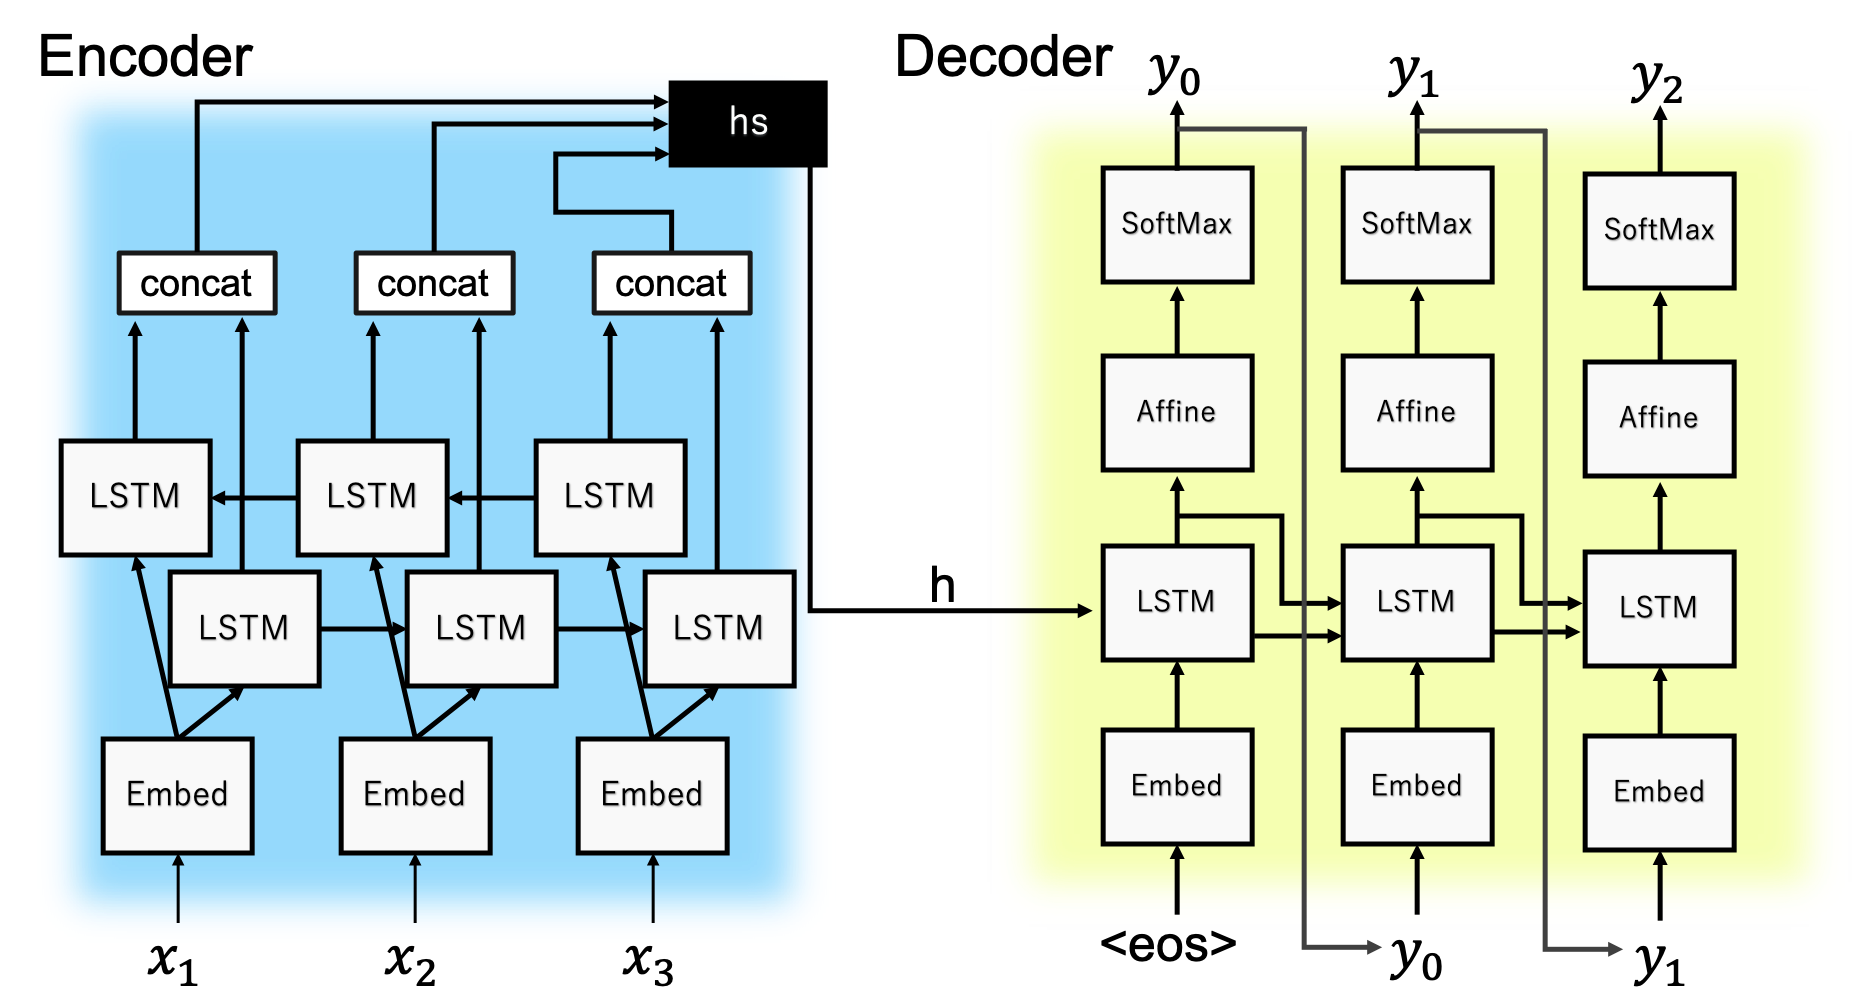
\includegraphics[width=\linewidth]{image/twinRNN.png}
      \caption{bi-directionl Seq2seq}
      \label{fig:bi-directionl Seq2seq}
    \end{minipage}

    %--- 中央スペース

    \begin{minipage}{0.06\hsize}
      \hspace{2mm}
    \end{minipage}


    \begin{minipage}{0.47\hsize}
      \centering
      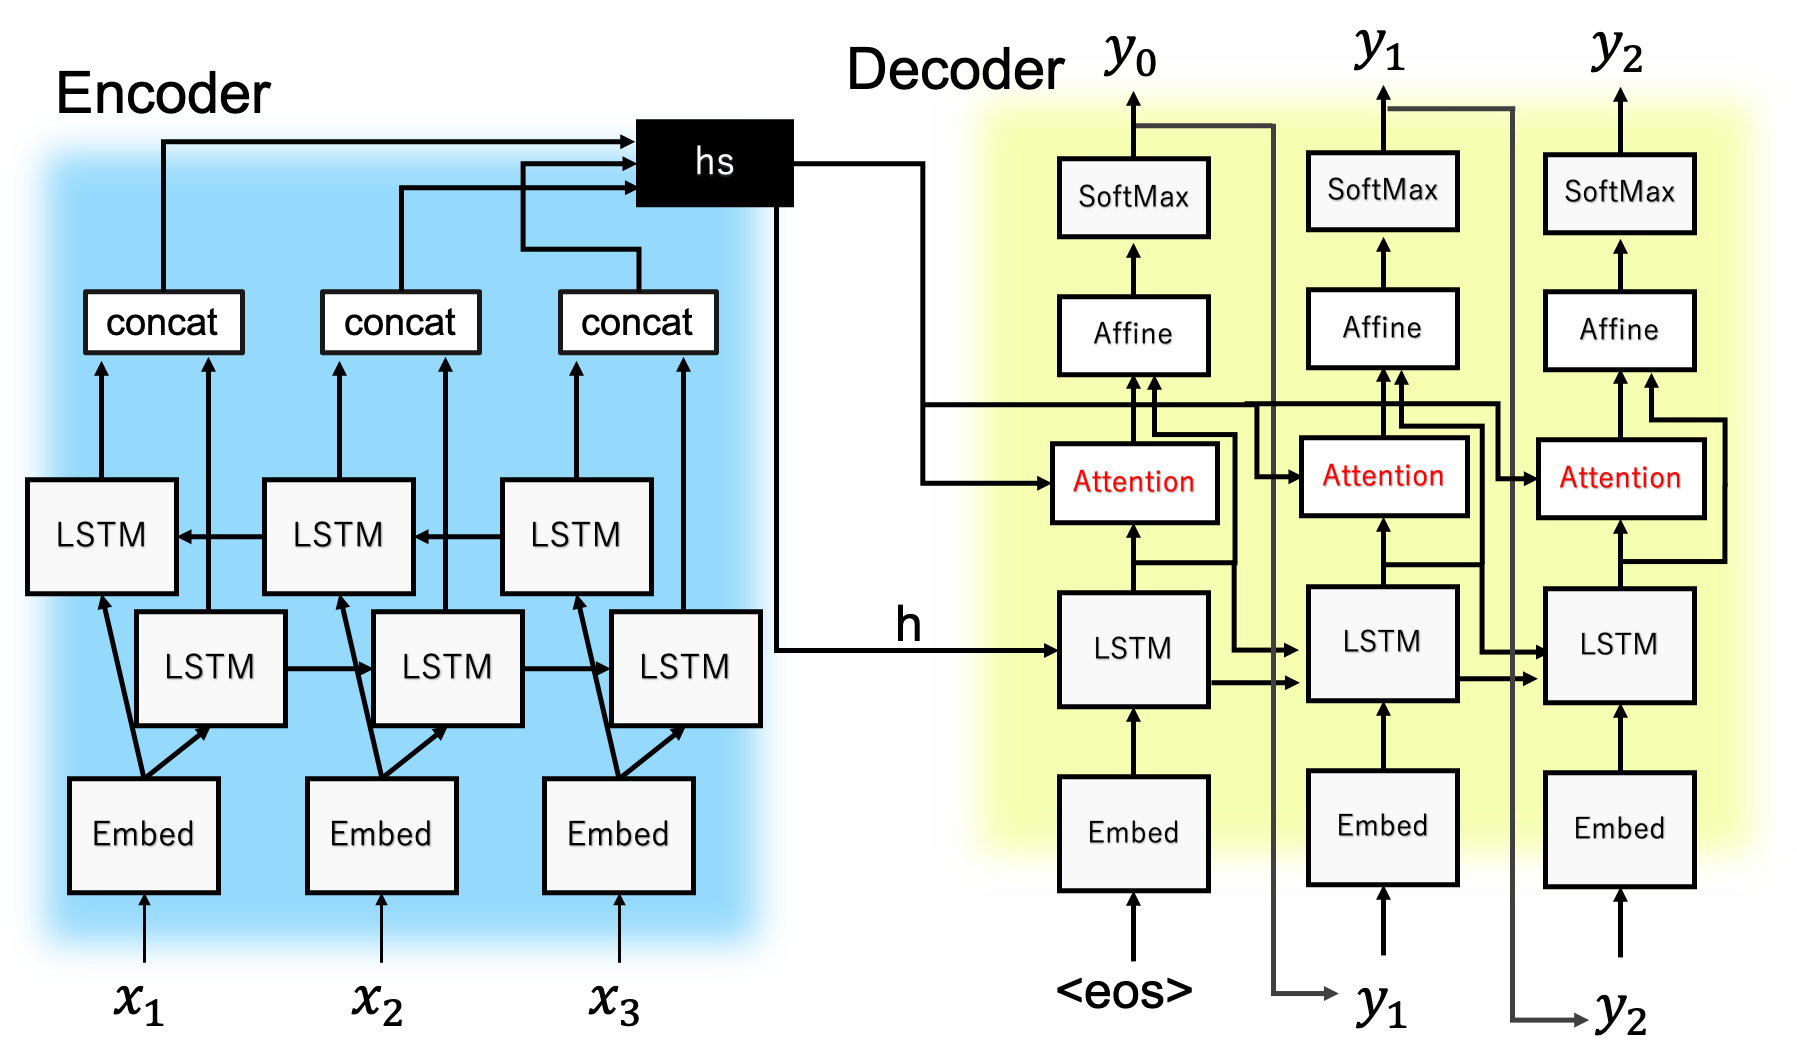
\includegraphics[width=\linewidth]{image/twinRNN2Attention.png}
      \caption{bi-directionlAttentionSeq2Seq}
      \label{fig:bi-directionl AttentionSeq2Seq}
    \end{minipage}

  \end{tabular}
\end{figure}


\begin{figure}[htpb]
  \centering
  \begin{tabular}{c}

    \begin{minipage}{0.47\hsize}
      \centering
      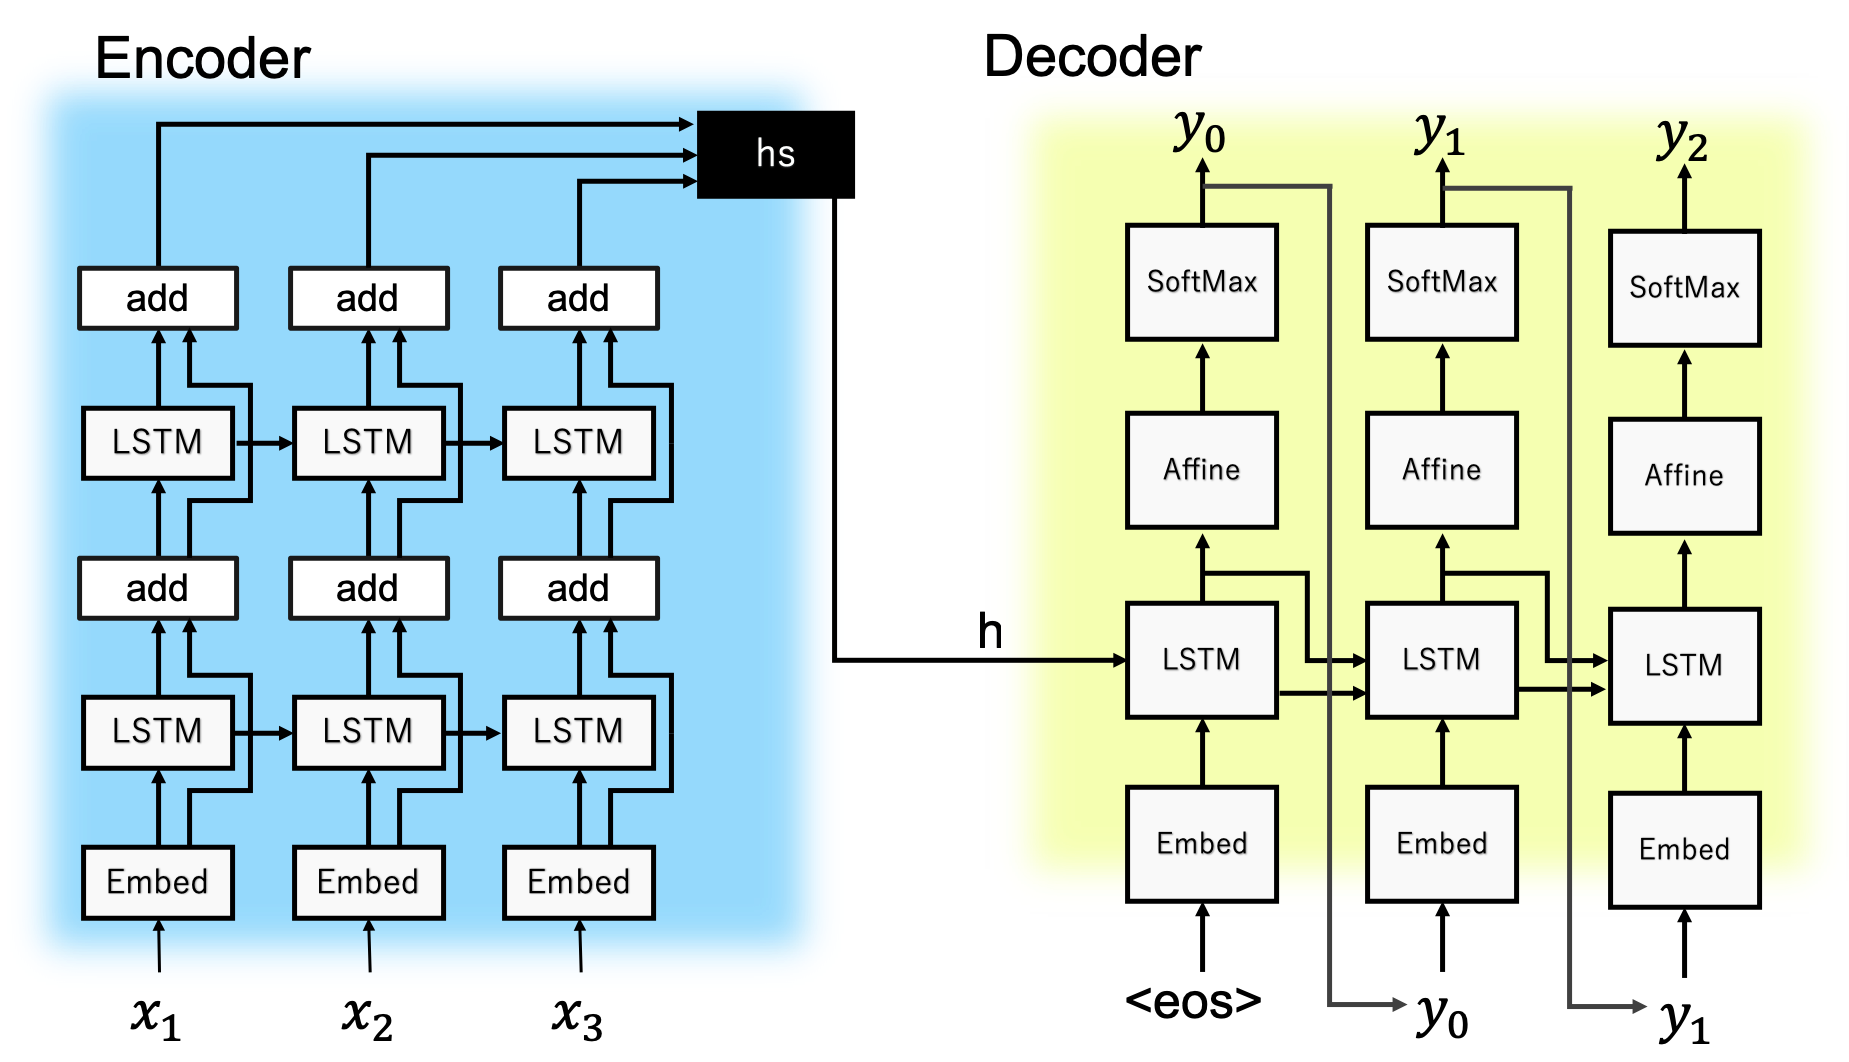
\includegraphics[width=\linewidth]{image/Skipconnect.png}
      \caption{Skip Seq2seq}
      \label{fig:SkipSeq2seq}
    \end{minipage}

    %--- 中央スペース

    \begin{minipage}{0.06\hsize}
      \hspace{2mm}
    \end{minipage}


    \begin{minipage}{0.47\hsize}
      \centering
      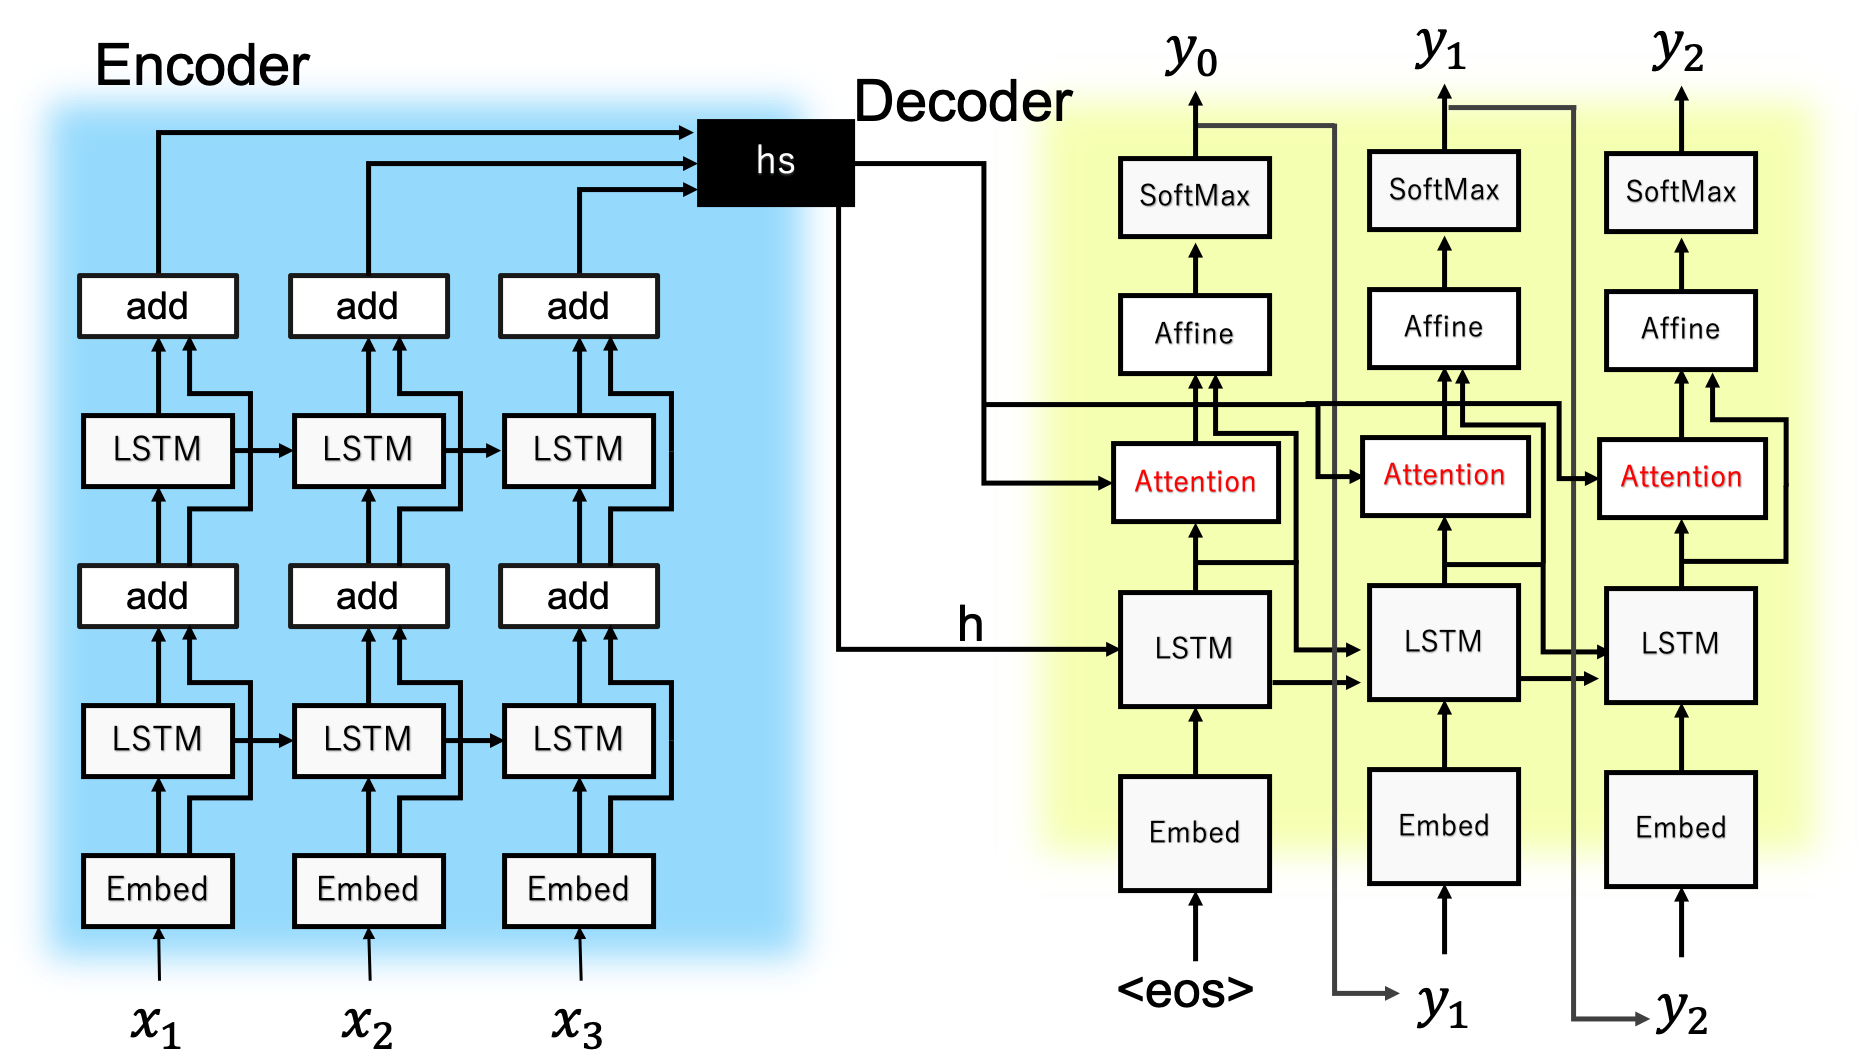
\includegraphics[width=\linewidth]{image/SkipAttention.png}
      \caption{Skip Attention Seq2Seq}
      \label{fig:SkipAttentionSeq2Seq}
    \end{minipage}

  \end{tabular}
\end{figure}

\clearpage
\section{正誤判定機}
\subsection{概要}
プリントから回答者の問題の正誤を判定し,記録していくのがOX Discriminaerである.
正誤を判定するのには画像認識のニューラルネットを利用している.回答用紙の答えのところを切り取り,各問題に対して正解か不正解かを確認し,別途用意した,個人のプリント進行表csvファイルにプリント番号とそのプリントの問題ごとを正解ならo,不正解ならxとしてファイルに書き込んでいく.(図\ref{fig:Discriminater_simple})

\begin{center}
  \begin{figure}[htb]
    \centering
    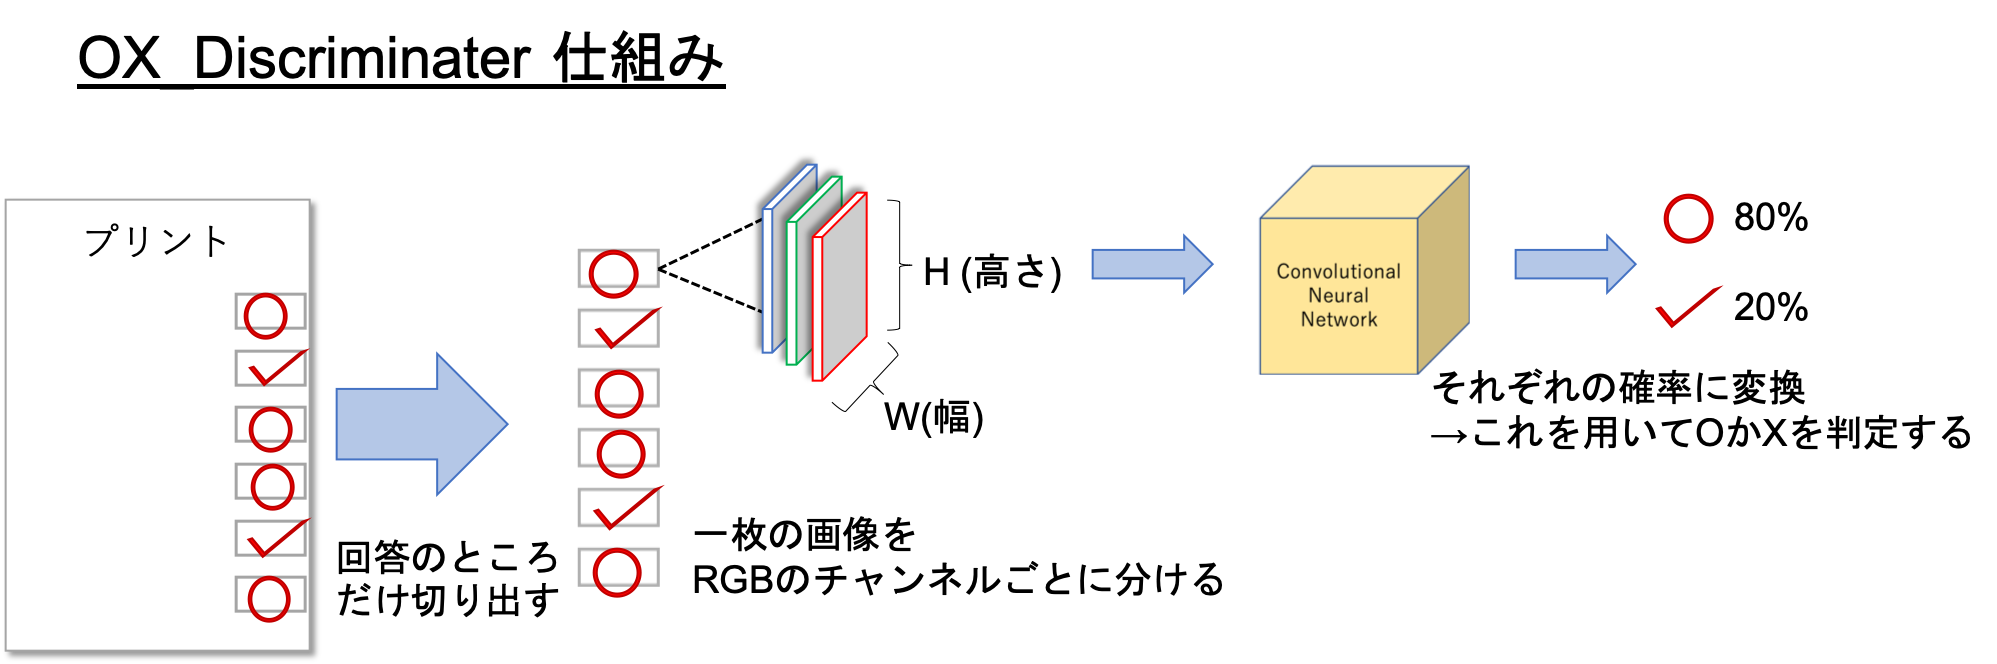
\includegraphics[width=\linewidth]{image/OX_Discriminater.png}
    \caption{OX Discriminater仕組み}
    \label{fig:Discriminater_simple}
  \end{figure}
\end{center}





\chapter{結果とその検討 \label{ch:result}}
\if0
\point{
自分の提案する方法が序論で提起した問題を解決できているかを評価・分析する.
\begin{itemize}
  \item 目的.何を確認するためのものか
  \item 方法.そのためにどういう実験を行ったか? 実験環境・用いたデータとその選定理由・手順を示し,評価の適切性を論証すること.
  \item 結果.その結果はどうだったか? 表やグラフを用いてまとめる.表はTeX,グラフはexcelでなくpythonを用いて作成すること.
  \item 分析.その結果から何が言えるか? 達成できた点・不足している点を理由と共に述べ,原因を考察する.
\end{itemize}
}
\fi

\section{実験}
以下の目的,方法,を元に実験を行った.
\subparagraph{計算式の特徴量抽出}
\begin{itemize}
  \item 目的.数式のベクトル表現は可能なのかどうか
  \item 方法.埋め込み層,ネットワーク構成を変えながらEncoder-Decoderで復元を試みる
  そのEncoderの出力値を数式ベクトルとしてみなし,pca,T-sneで二次元ベクトルに圧縮し図示する
\end{itemize}

実験で試したネットワーク構成は以下の通りである.


\begin{table}[hbt]
  \begin{center}
    \caption{Encorderの構成}
    \label{table:Encorder}
    \begin{tabularx}{0.9\linewidth}{|l|l|X|}
      \hline
      1 & Embedding層 & 入力ノード数:$89$,出力ノード数:$2$ \\
      \hline
      2 & LSTM層 & 入力ノード数:$2$,出力ノード数:$50$ \\
      \hline
      3 & LSTM層 & 入力ノード数:$50$,出力ノード数:$50$ \\
      \hline
    \end{tabularx}
  \end{center}
\end{table}


\begin{table}[hbt]
  \begin{center}
    \caption{Encorderの構成}
    \label{table:Decorder}
    \begin{tabularx}{0.9\linewidth}{|l|l|X|}
      \hline
      1 & Embedding層 & 入力ノード数:$89$,出力ノード数:$2$ \\
      \hline
      2 & LSTM層 & 入力ノード数:$2$,出力ノード数:$50$ \\
      \hline
      3 & LSTM層 & 入力ノード数:$50$,出力ノード数:$50$ \\
      \hline
      4 & LSTM層 & 入力ノード数:$50$,出力ノード数:$50$ \\
      \hline
      4 & Affine層 & 入力ノード数:$50$,出力ノード数:$89$ \\
      \hline
    \end{tabularx}
  \end{center}
\end{table}
\clearpage

\section{実験結果}
以下ネットワーク\ref{table:Encorder},\ref{table:Decorder}で学習データ10個を学習し,Encoderの出力の式の分散表現と思われるものの分布である.
学習データは以下の10個である.
\begin{itemize}
  \item\verb#x+5=8#
  \item\verb#5x-7=4#
  \item\verb#3.6+x=-1.4#
  \item\verb#3x-4=-5x+5#
  \item\verb#\frac{7}{2}x+9=6#
  \item\verb#3(2x-1)=9#
  \item\verb#\frac{3}{7}x+2=\frac{6}{7}#
  \item\verb#-\frac{4}{7}x+3=-\frac{1}{7}x#
  \item\verb#\frac{x+1}{3}+\frac{2x+1}{2}=\frac{3x-4}{2}#
  \item\verb#-4x+9=1#
\end{itemize}


\begin{center}
  \begin{figure}
    \centering
    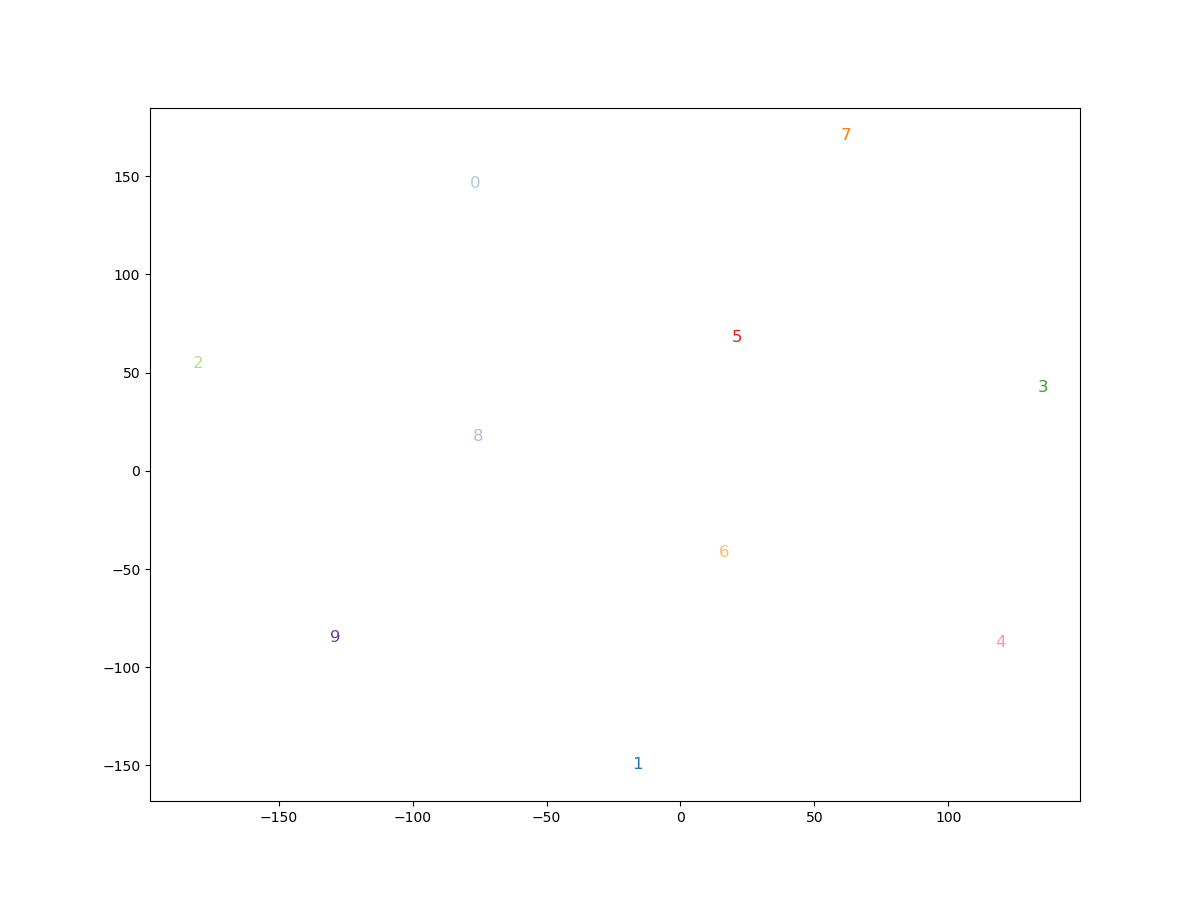
\includegraphics[width=0.8\linewidth]{image/cbow89x2.png}
    \caption{式ベクトルの分布(cbow)}
    \label{fig:formulavecter_fromCbow}
  \end{figure}
\end{center}


\begin{center}
  \begin{figure}
    \centering
    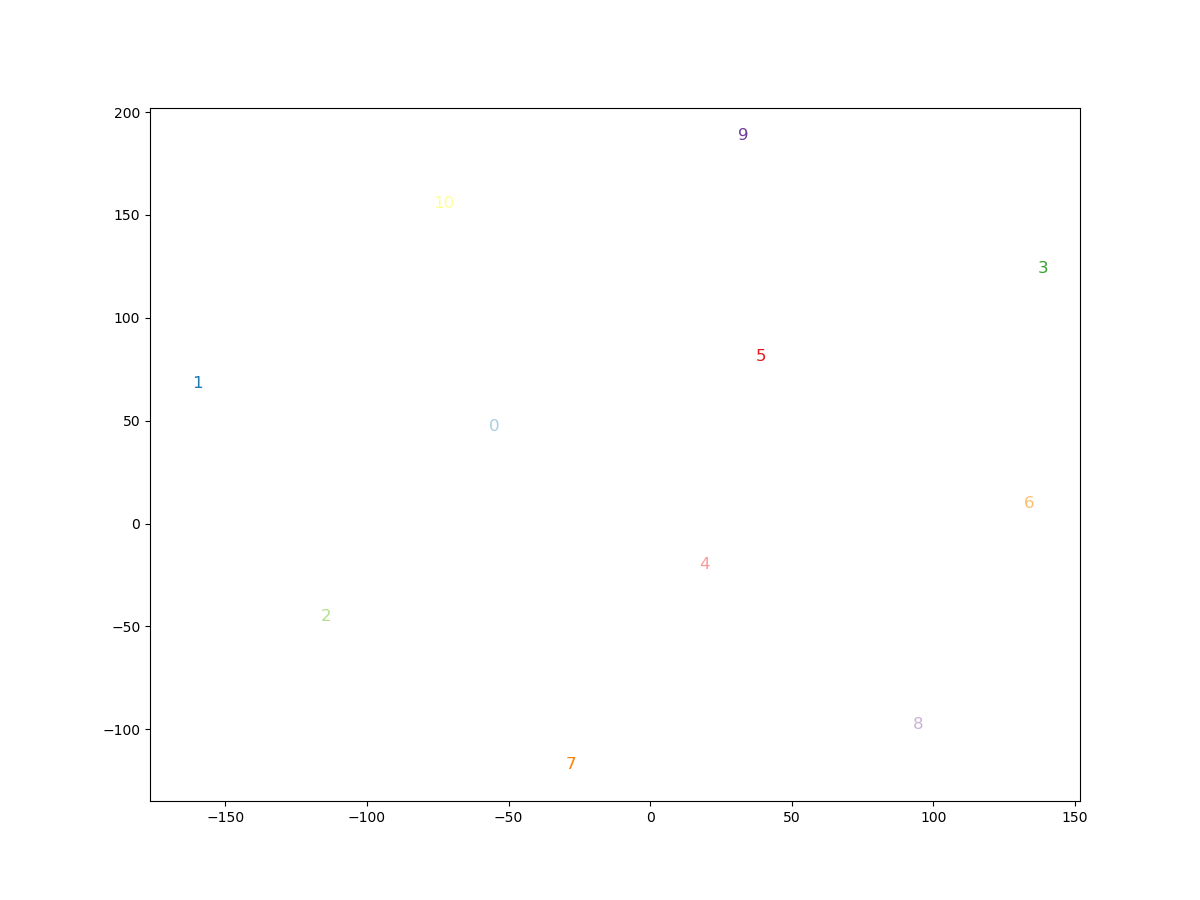
\includegraphics[width=0.8\linewidth]{image/skip89x2.png}
    \caption{式ベクトルの分布(skipgram)}
    \label{fig:formulavecter_fromSkip}
  \end{figure}
\end{center}

\section{考察}
結果の図\ref{fig:formulavecter_fromCbow},図\ref{fig:formulavecter_fromSkip}は結果としてどちらも特徴をとらえていない結果となった.
考えれる原因として,LSTMでは入力された順番の情報は残らないため前後の関係に強く依存する数式ではうまく表現できなかったように思える
よって,今後は双方向LSTMやAttentionを用いて前後の関係と,どこに注目してエンコードするのかを強化するひち用がある.
また,LSTMの隠れ層を深くすることも考えられるが,過学習が起きてしまうためDropoutなど正則化を行い,学習を進める必要がある.


\if0
\subparagraph{計算式の特徴量からの類題選出}
\begin{itemize}ß
  \item 目的.求めた計算式のベクトルから特徴を捉えた数式を選出できるか
  \item 方法.特徴量ベクトルからk近法で選出,ある生徒の間違えた一問から類題を選出し,実際にその問題を間違えていたかを確認,また,逆にあっていた問題からも同様な手法で確認

\end{itemize}
\fi
\subsection{問題の正誤判定}
研究室の同期メンバーの手書きによる訓練データ927件,実際の子供たちの手書きによるテストデータ197件にて学習を行った.
正解率(図\ref{fig:OX_Discriminater_ACC}),平均二乗誤差(図\ref{fig:OX_Discriminater_loss})を示す.

\begin{center}
  \begin{figure}
    \centering
    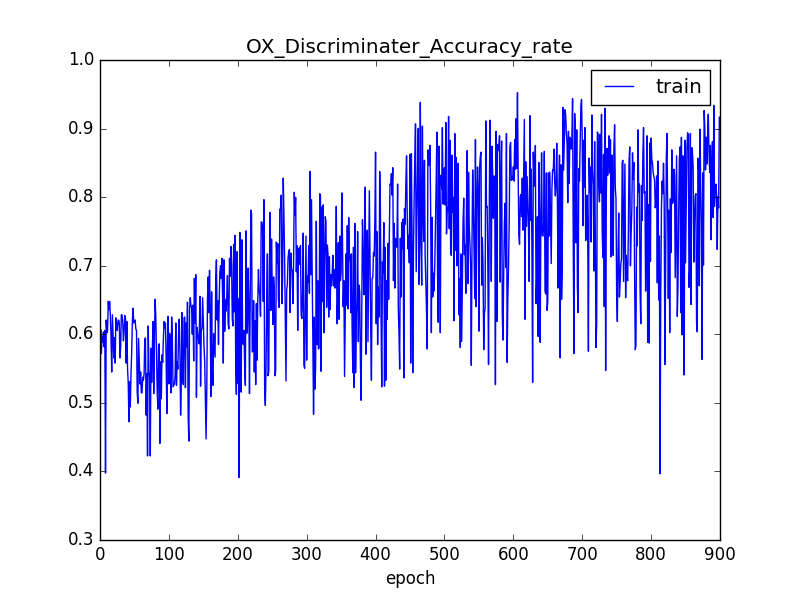
\includegraphics[width=0.8\linewidth]{image/OX_Discriminater_Accuracy_rateplot.png}
    \caption{OX Discriminater 正解率}
    \label{fig:OX_Discriminater_ACC}
  \end{figure}
\end{center}


\begin{center}
  \begin{figure}
    \centering
    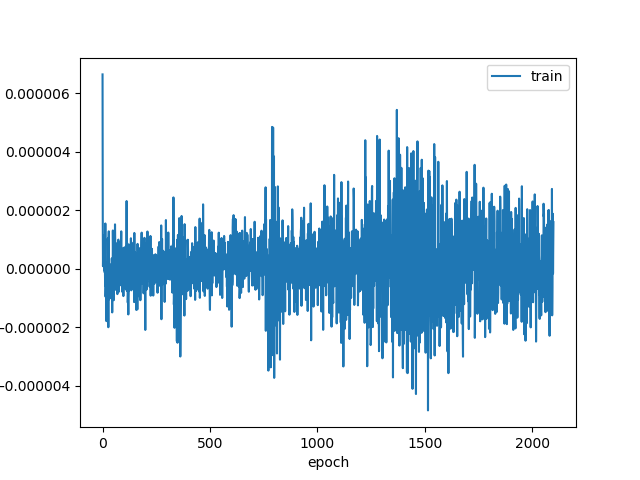
\includegraphics[width=0.8\linewidth]{image/LOSSplot.png}
    \caption{OX Discriminater 平均二乗誤差 }
    \label{fig:OX_Discriminater_loss}
  \end{figure}
\end{center}
\clearpage








\chapter{関連研究\label{ch:relsatedwork}}
自然言語処理を数式を適応した例は筆者が調べるかぎりはなく,自然言語以外にWord2vecを適用しようとした研究はいくつかあり,再帰ニューラルネットを応用したものである.
文献\cite{kannrenn3}では文の特徴をEncoder-Decoderの機構を用いて学習し,Encoderの隠れ層の出力により文章の類似度を算出している.文献\cite{kannrenn3}によると小説の一部を学習データに用いて,埋め込み層としてSkipGramを適用している.gemsimのDoc2Vecとの比較がなされているが,ユーザーにとって有益な評価方法の設定の難しさを述べている.

文献\cite{lannrenn4}ではプログラムコードを埋め込み,再構成して実行できるかどうかを試している.C言語で書かれたプログラムを一文字ごと,i-of-k符号化して読み込んでいる.Dropoutを適用させることにより性能を向上させている.今後,スペルミスによるコンパイルエラーを事前に直してくれることを目的としている.

文献\cite{kannrenn5}ではDeepLearingの技術の検索の際,ユーザーが求めている情報を推奨することを目的としている.
評価方法としてMovie Lens-100Kでの映画の推奨をパラメーター,ネットワークの構成を様々試しながら知見を集めている.
AEは層を重ねても,性能は向上せず,各映画のユーザー平均を差し引いて正規化しても低脳は大きく変化しない.
これにより,特徴抽出の重要さを筆者は述べている.





\chapter{結論と今後の課題 \label{ch:conclusion}}
\if0
\point{
序論で提起した問いとそれに対する答えをまとめる.
\begin{itemize}
  \item 提案手法のアイデアおよび評価結果を振り返る.
  \item この研究で得られた知見をまとめる.
  \item 今後の課題について述べる.
\end{itemize}
}
\fi

本研究の結果によって計算式をベクトルとして扱うことが可能なことが示唆することができた.
これにより数式データのみで最適な問題選択を可能とし,いまある個人情報と合わせるとより高い精度でシステムが提供できるように思う.
本研究により,自然言語処理の分野で発展してきた技術は人口言語でも利用することができることが示せた.
これは人間が作り発展させてきたものはどこか本質的には同様の特徴を持っており,その特徴をコンピュータが学ぶことができたことではないだろうか.

しかしながら,未だ問題点はあり,計算問題には簡約な問題ほどパターンがなくなり,式から有用な情報が取り出せなくなる恐れがある.
また,多くの子供が苦手とする文章題は本研究では扱っていないが,Dec2Vecなど文章をベクトル化する手法は提案されており,それを応用することにより可能性は広がるだろう.
また,本研究で扱った一次方程式の特徴量を使って別の分野を分類し,個人のまちがえた問題の情報を元に転移学習を行うとより,包括的なアダプティブラーニングシステムの構築が行えるようになり自分で学ぶ際の道しるべとなることを期待している.



\if0
\chapter{形式上の注意}

\begin{itemize}
  \item 文字コードはUTF-8に統一する.
  \item 論文ファイル名は\texttt{chishiro-thesis.tex},文献ファイル名は\texttt{chishiro.bib}のように名前\texttt{-thesis.tex}とする.
  \item 句読点は全角のカンマ,ピリオドを用いる.
  \item 英数字はすべて半角を用いる.ギリシャ文字は{\TeX}の定義を用いる.$\alpha, \beta, ...$
  \item カンマの前にはスペースを入れず,カンマの後はスペースをひとつ入れる.
  \item 数式は{\TeX}の数式機能を用いる.例: $x^2$,\[f(x) = x^2 + 2x + 1.\].
  \item プログラムテキストはタイプライターフォントを用いる(例: \texttt{hello}).
  \item 文章構成(章・節・小節・箇条書き)は{\TeX}の機能を用いて指定する.自分で見出しなどを作らない.
  \item 題目には研究目的・方法・対象を特徴づける情報を入れる.
  \item 図のタイトルは図の下,表のタイトルは表の上に書く.
  \item 図表番号の参照は\verb#\label#および\verb#\ref#を用いる.自分で図表番号を指定しない.
  \item 表は{\TeX},グラフはすべてpythonで作成する.
  \item 図表番号のない図は用いない.
  \item 参照の?は必ず取り除く.
  \item 段落は意味の区切りでわける.意図しない字下げが入った場合\verb#\noindent#を用いて修正する.
  \item 参考文献は10以上あげる.
\end{itemize}
\fi


\chapter*{謝辞 \label{ch:acknowledgement}}
\thispagestyle{empty}
\if
\point{
本のあとがきに相当する部分.半ページ 以上書く.
卒業研究に協力者してくれた方々へのお礼を忘れずに述べる.
}
\fi
この研究を進めるにあたって,私の興味の赴くまま進める中,様々な角度からご指導いただいた千代教授に深く感謝申し上げます.
また研究が,会話を通して気づきを与えてくれた同研究室メンバーに感謝申し上げます.
最後に,毎週たくさんの計算問題を宿題として解いてきてくれた私の塾の生徒たちに感謝をするとともに
必ず,この経験を元に世の中により良い教育システムを提供し今まで手の届かなかった子供達の未来に手助けすることを約束し,謝辞といたします.


\bibliography{miyaji}
\end{document}
